\chapter[Detection of copropagating beams]{Detection of copropagating beams}\label{chapter:copropagating_beams}


\section[Electromagnetic field of relativistic charged particles]{Electromagnetic field of relativistic charged particles}


Relativistic effects induce substantial modifications to the electromagnetic field radiated by charged particles. It is therefore necessary to understand how the field distribution is modified when it is observed in different reference frames.

Consider two inertial reference frames to study the field of a charged particle in uniform motion. In the rest frame $\Sigma'$, the particle velocity is zero. The electric field of the particle is isotropic, and the field magnitude is expressed as
\begin{equation}
E(r) = \frac{1}{4\pi\epsilon_0} \frac{q}{r^2}
\end{equation}
where $q$ is the particle's electric charge, $r$ is the distance between the observation point and the particle  and $\epsilon_0$ is the dielectric constant of vacuum. 

The laboratory frame $\Sigma$ sees the particle and the rest frame in motion with a relative velocity $v = \beta c$, where $\beta$ is the particle speed in units of the speed of light in vacuum~$c$. The Lorentz factor is defined as 
\begin{equation}
    \gamma = \frac{1}{\sqrt{1-\beta^2}}
\end{equation}
where $\gamma = 1$ corresponds to zero velocity and $\gamma \rightarrow \infty$ as the velocity approaches the speed of light.


\begin{figure}[!t]
\centering
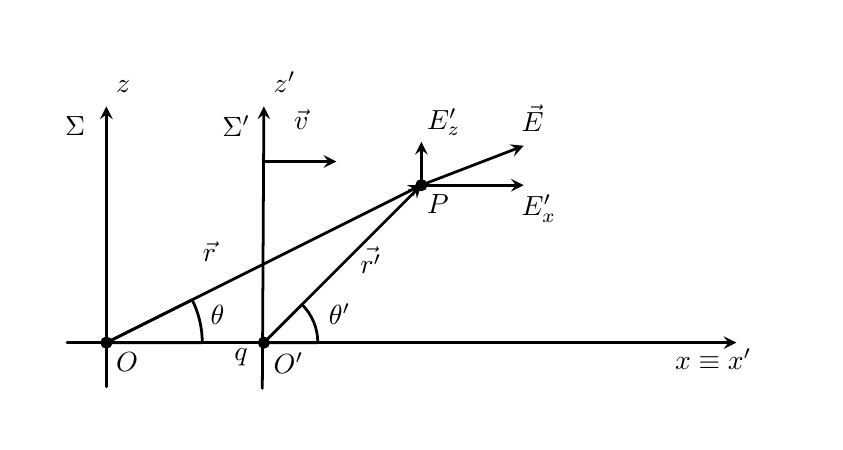
\begin{tikzpicture}[line cap=round,line join=round,>=stealth,x=1cm,y=1cm]

\clip(-1,-1) rectangle (9, 4);

\draw [->,line width=1pt] (0,-0.56) -- (0,3);
\draw [->,line width=1pt] (-0.5,0) -- (8,0);
\draw [->,line width=1pt] (1.98,-0.58) -- (2,3);
\draw [->,line width=1pt] (4,2) -- (5.3,2);
\draw [->,line width=1pt] (4,2) -- (4.,2.55);
\draw [->,line width=1pt] (0,0) -- (4,2);
\draw [->,line width=1pt] (2,0) -- (4,2);
\draw [->,line width=1pt] (4,2) -- (5.3,2.5);
\draw [->,line width=1pt] (2,2.3) -- (2.92,2.3);

\draw (-0.65,3.) node[anchor=north west] {$\Sigma$};
\draw (7.0985076482125695,0.04219672712700242) node[anchor=north west] {$x \equiv x'$};
\draw (2.,3.05) node[anchor=south west] {$z'$};
\draw (0.,3.05) node[anchor=south west] {$z$};
\draw (1.35,3.) node[anchor=north west] {$\Sigma'$};
\draw (2.258296995869005,3.0833910308119017) node[anchor=north west] {$\vec{v}$};
\draw (3.100693540082192,1.3414863122693772) node[anchor=north west] {$\vec{r'}$};
\draw (1.1,1.4) node[anchor=north west] {$\vec{r}$};
\draw (1.5,0.05) node[anchor=north west] {$q$};
\draw (3.95,2.) node[anchor=north west] {$P$};
\draw (5.15,2.) node[anchor=north west] {$E'_x$};
\draw (3.95,3.1) node[anchor=north west] {$E'_z$};
\draw (5.15,3.15) node[anchor=north west] {$\vec{E}$};

\draw (0,0) node[anchor=north west] {$O$};
\draw (2,0) node[anchor=north west] {$O'$};

\draw (1.2,0.1) node[anchor=south west] {$\theta$};
\draw (2.7,0.1) node[anchor=south west] {$\theta'$};

\draw [shift={(0,0)},line width=1pt,color=black,fill=black,fill opacity=0.] (0,0) -- (0:1.2172923398962883) arc (0:26.56505117707799:1.2172923398962883) -- cycle;
\draw [shift={(2,0)},line width=1pt,color=black,fill=black,fill opacity=0.] (0,0) -- (0:0.6847269411916621) arc (0:45:0.6847269411916621) -- cycle;


\begin{scriptsize}
\draw [fill=black] (0,0) circle (2pt);
\draw [fill=black] (2,0) circle (2pt);
\draw [fill=black] (4,2) circle (2pt);
\end{scriptsize}

\end{tikzpicture}
\caption{Schematic representation of the reference frames. The laboratory frame $\Sigma$ and the particle rest frame $\Sigma'$ are shown. }
\label{fig:frames}
\end{figure}

Figure~\ref{fig:frames} shows a schematic representation of the two reference frames. The charge $q$ is placed in the origin $O'$ of the rest reference frame $\Sigma'$. The distances between the field observation point $P$ and the origins of rest and laboratory reference frames are indicated with $\vec{r}$ and $\vec{r'}$, respectively. 

For a relativistic motion in the $x$ direction, there is a time~$t_0$ when the particle is at the origin $O$, and the origins of the reference frames $\Sigma$ and $\Sigma'$ coincide. The electric field in the observation point $P$, when observed from the origin of the laboratory frame $\Sigma$ is expressed as~\cite{Jackson:490457}:
\begin{equation}
E\left( \theta \right) = \frac{q}{r^2 \gamma^2} \frac{1}{\left( 1 - \beta^2 sin^2\left(\theta\right) \right)^\frac{3}{2}}
\end{equation}
The two limit cases:
\begin{equation}
    E\left( \theta = \frac{\pi}{2} \right) = \frac{q \gamma}{r^2 }\label{eq:pi/2}
\end{equation}
\begin{equation}
    E\left( \theta = 0 \right) = \frac{q }{r^2 \gamma^2}\label{eq:zero}
\end{equation}
are the electric fields in the direction of motion and in the normal direction. These expressions have some important implications. A static particle (or observed in its rest frame) presents the same electric field in the perpendicular and parallel direction of motion, as the field is isotropically distributed. As soon as the particle is in motion, the transverse field increases by a factor of $\gamma^3$ with the field in the direction of motion suppressed by $1/\gamma$. As the particle approaches the speed of light, its electric field is therefore almost only transverse. This effect is shown in Fig.~\ref{fig:field_pattern} presenting the electric field spatial distribution for particles with increasing velocities. The field lines become denser in the direction perpendicular to the motion. In the ultra-relativistic limit, the angle of the field lines becomes very narrow, and the particle field is approximately transverse to the direction of motion.



\begin{figure}[!h]
\centering
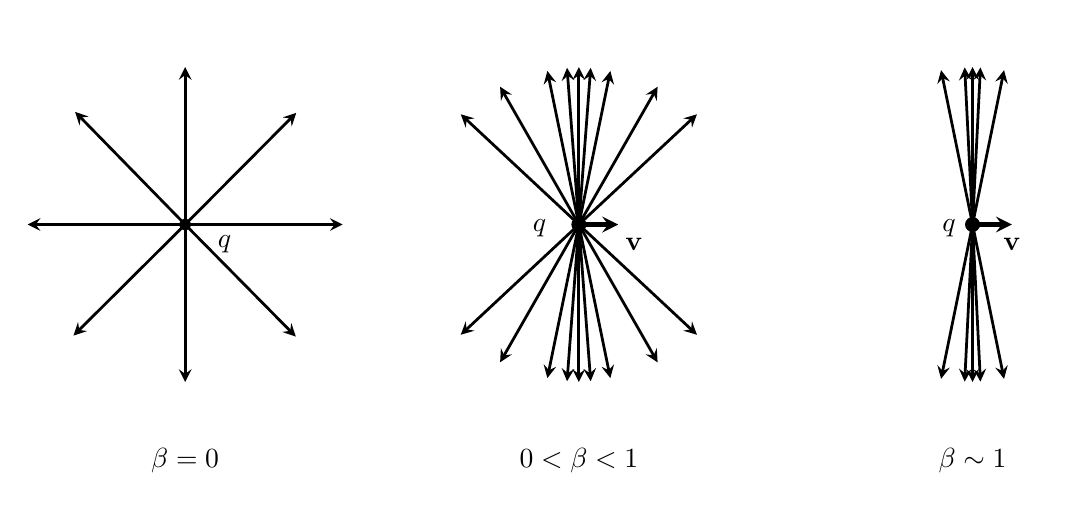
\begin{tikzpicture}[line cap=round,line join=round,>=stealth,x=1cm,y=1cm]
\clip(-2.,-3.5) rectangle (11,2.5);
\draw [->,line width=1pt] (0,0) -- (-1.3975053304790308,1.4307266864368944);
\draw [->,line width=1pt] (0,0) -- (0,2);
\draw [->,line width=1pt] (0,0) -- (1.41035916900663,1.4180574792295721);
\draw [->,line width=1pt] (0,0) -- (2,0);
\draw [->,line width=1pt] (0,0) -- (1.4051129272120964,-1.4232560071123728);
\draw [->,line width=1pt] (0,0) -- (0,-2);
\draw [->,line width=1pt] (0,0) -- (-1.4180074832552354,-1.4104094360972468);
\draw [->,line width=1pt] (0,0) -- (-2,0);

\draw [->,line width=1pt] (5,0) -- (3.5,1.4);
\draw [->,line width=1pt] (5,0) -- (6.5,1.4);
\draw [->,line width=1pt] (5,0) -- (3.5,-1.4);
\draw [->,line width=1pt] (5,0) -- (6.5,-1.4);
\draw [->,line width=1pt] (5,0) -- (5,2);
\draw [->,line width=1pt] (5,0) -- (5,-2);
\draw [->,line width=1pt] (5,0) -- (4.6,-1.95);
\draw [->,line width=1pt] (5,0) -- (5.4,-1.95);
\draw [->,line width=1pt] (5,0) -- (4.6,1.95);
\draw [->,line width=1pt] (5,0) -- (5.4,1.95);

\draw [->,line width=1pt] (5,0) -- (4.85,-1.99);
\draw [->,line width=1pt] (5,0) -- (5.15,-1.99);
\draw [->,line width=1pt] (5,0) -- (4.85,1.99);
\draw [->,line width=1pt] (5,0) -- (5.15,1.99);

\draw [->,line width=1pt] (5,0) -- (6.,1.75);
\draw [->,line width=1pt] (5,0) -- (4.,1.75);
\draw [->,line width=1pt] (5,0) -- (4.,-1.75);
\draw [->,line width=1pt] (5,0) -- (6.,-1.75);


\draw [->,line width=1pt] (10,0) -- (10,2);
\draw [->,line width=1pt] (10,0) -- (10,-2);
\draw [->,line width=1pt] (10,0) -- (10.4,1.96);
\draw [->,line width=1pt] (10,0) -- (9.6,-1.96);
\draw [->,line width=1pt] (10,0) -- (10.1,1.995);
\draw [->,line width=1pt] (10,0) -- (9.9,1.995);
\draw [->,line width=1pt] (10,0) -- (9.9,-1.995);
\draw [->,line width=1pt] (10,0) -- (10.1,-1.995);
\draw [->,line width=1pt] (10,0) -- (9.6,1.96);
\draw [->,line width=1pt] (10,0) -- (10.4,-1.96);

\draw (0,-3) node[anchor=center] {$\beta =0$};
\draw (5, -3) node[anchor=center] {$ 0 < \beta < 1$};
\draw (10,-3) node[anchor=center] {$\beta \sim 1$};

\draw (0.5,-0.25) node[anchor=center] {$q$};
\draw (4.5,-0.05) node[anchor=center] {$q$};
\draw (9.7,-0.05) node[anchor=center] {$q$};

\draw [->,line width=1.5pt] (10,0) -- (10.5,0);
\draw (10.5, -0.25) node[anchor=center] {$\mathbf{v}$};
\draw [->,line width=1.5pt] (5,0) -- (5.5,0);
\draw (5.7, -0.25) node[anchor=center] {$\mathbf{v}$};



\begin{scriptsize}
\draw [fill=black] (0,0) circle (2pt);
\draw [fill=black] (10,0) circle (2.5pt);
\draw [fill=black] (5,0) circle (2.5pt);
\end{scriptsize}

\end{tikzpicture}
\caption{Schematic representation of the spatial field distribution for a charge $q$ at rest ($\beta=0$) and at increasing velocities.}
\label{fig:field_pattern}
\end{figure}



In general, the transformation of the electric and magnetic field from an arbitrary frame $\Sigma$ to another $\Sigma'$ in motion with a relative velocity~$\mathbf{v}$ is expressed by the following relations~\cite{Jackson:490457}:
\begin{equation}
\mathbf{E'} = \gamma \left( \mathbf{E} + \mathbf{\beta} \times \mathbf{B} \right) -\frac{\gamma^2}{\gamma +1} \mathbf{\beta} \left( \mathbf{\beta} \cdot \mathbf{E}  \right)
\end{equation}
\begin{equation}
\mathbf{B'} = \gamma \left( \mathbf{B} + \beta \times \mathbf{E} \right) -\frac{\gamma^2}{\gamma +1} \beta \left( \beta \cdot \mathbf{B}  \right)
\end{equation}
Therefore, a purely electric or magnetic field can exist only in the rest frame (where $\beta=0$), but becomes a mixture of the two as soon as they are observed from a different frame. 






\section[Signal generation in a capacitive BPM]{Signal generation in a capacitive BPM}


\subsection[Wall currents]{Wall currents}

In particle accelerators, a beam of charged particles typically travels through a metal beampipe inducing an image charge on the conductive walls. In the ultra-relativistic limit, the particles' field is transverse to the motion direction. Therefore, the image charge on the beampipe walls will form a section of a cylinder that follows the beam particles. The total electric current induced on the beampipe walls, called the wall current, will be equal to the beam current but will have the opposite polarity. Assuming the beam is in the centre of a perfectly conducting cylindrical beampipe, the wall current distribution $i_\text{wall}$ along the circumference is
\begin{equation}
i_\text{wall}(t) = -\frac{I_\text{beam}(t)}{2\pi b}
\end{equation}
where $I_\text{beam}$ is the beam current and $b$ is the beampipe radius. 


\begin{figure}[!b]
\centering
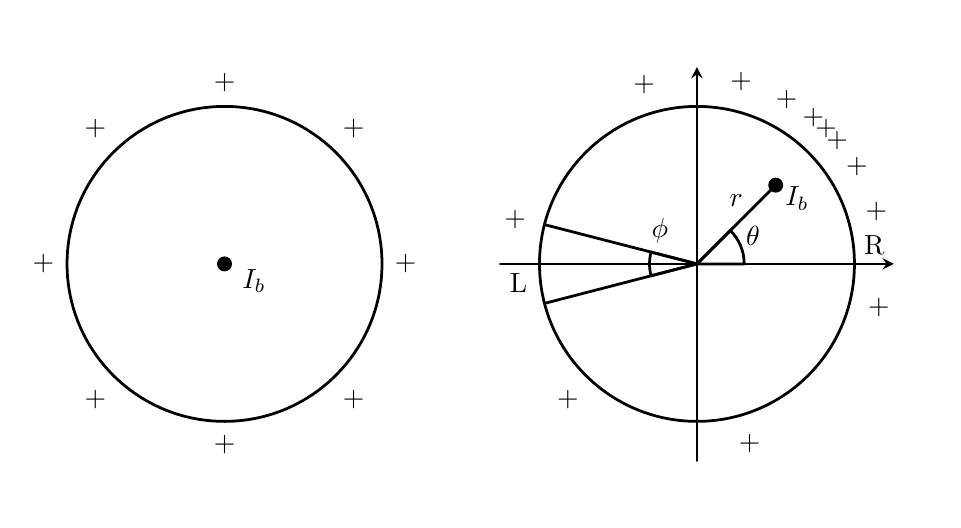
\begin{tikzpicture}[line cap=round,line join=round,>=stealth,x=1cm,y=1cm]
\clip(-0.5,-3) rectangle (11,3);

% first circle
\draw [line width=1pt] (2,0) circle (2cm);
\draw (2.102339116057103,0.049046415693315894) node[anchor=north west] {$I_b$};
\draw [fill=black] (2,0) circle (2.5pt);

\draw (-0.3,0) node[anchor=center] {$+$};
\draw (4.3,0) node[anchor=center] {$+$};
\draw (2,2.3) node[anchor=center] {$+$};
\draw (2,-2.3) node[anchor=center] {$+$};

\draw (0.36,1.72) node[anchor=center] {$+$};
\draw (0.36,-1.72) node[anchor=center] {$+$};
\draw (3.64,1.72) node[anchor=center] {$+$};
\draw (3.64,-1.72) node[anchor=center] {$+$};

% second circle


\draw [fill=black] (9,1) circle (2.5pt);
\draw [line width=1pt] (8,0) circle (2cm);

\draw [->,line width=0.8pt] (8,-2.5) -- (8,2.5);
\draw [->,line width=0.8pt] (5.5,0) -- (10.5,0);
% \draw (10.4,0.1) node[anchor=north west] {$x$};
% \draw (8.05,3) node[anchor=north west] {$y$};

\draw [shift={(8,0)},line width=1pt,fill=black,fill opacity=0] (0,0) -- (0:0.6) arc (0:45:0.6) -- cycle;
\draw [shift={(8,0)},line width=1pt,fill=black,fill opacity=0] (0,0) -- (165.55343672100963:0.6024446573006162) arc (165.55343672100963:194.52396626116362:0.6024446573006162) -- cycle;

\draw [line width=1pt] (8,0)-- (9,1);
\draw (9,1.1) node[anchor=north west] {$I_b$};
\draw (8.5,0.6) node[anchor=north west] {$\theta$};
\draw (8.5,0.8) node[anchor=center] {$r$};
\draw (7.3,0.7) node[anchor=north west] {$\phi$};
\draw [line width=1pt] (6.063238529254589,0.4989539111341559)-- (8,0);
\draw [line width=1pt] (8,0)-- (6.063914351618504,-0.5015698975528741);

\draw (9.64,1.72) node[anchor=center] {$+$};
\draw (9.48,1.86) node[anchor=center] {$+$};
\draw (9.78,1.57) node[anchor=center] {$+$};
\draw (9.14,2.09) node[anchor=center] {$+$};
\draw (10.03,1.24) node[anchor=center] {$+$};

\draw (10.28,0.67) node[anchor=center] {$+$};
\draw (8.56,2.31) node[anchor=center] {$+$};
\draw (7.33,2.28) node[anchor=center] {$+$};
\draw (10.31,-0.56) node[anchor=center] {$+$};

\draw (6.36,-1.72) node[anchor=center] {$+$};
\draw (5.69,0.56) node[anchor=center] {$+$};
\draw (8.67,-2.28) node[anchor=center] {$+$};

\draw (5.5,0) node[anchor=north west] {L};
\draw (10,0) node[anchor=south west] {R};


\end{tikzpicture}
\caption{Charge distribution on the beampipe walls for an ultra-relativistic beam. On the left, the case for a centred beam, while on the right the beam is displaced. The induced image charges are schematically indicated with a + sign.}
\label{fig:wall_current}
\end{figure}




On the other hand, an off-centred beam will cause a redistribution of the image charge density. In the regions closer to the beam, a larger part of the total charge is induced. The different image charge formation in a transverse section of the beampipe is shown in Fig.~\ref{fig:wall_current}. The wall current distribution can be calculated using the image method~\cite{scharfer:bpm}:
\begin{equation}
i_\text{wall} (r, \theta, \phi, b; t) = -\frac{I_\text{beam}(t)}{2\pi b} \left[ \frac{b^2 - r^2}{b^2 + r^2 - 2br cos\left( \phi - \theta \right)}   \right] \label{eq:curr_dens}
\end{equation}
where $b$ is the beampipe radius, $r$ and $\theta$ are the polar coordinates that define the beam position and $\phi$ is the angular section of the wall considered in the calculation. For any fixed angle~$\phi$, a current $I_\text{L}$ can be obtained by integrating Equation~\ref{eq:curr_dens} (see Fig.~\ref{fig:wall_current}). Similarly, if we consider the opposite section, i.e. ~$\phi-180^\circ$ one can defined a current~$I_\text{R}$.

The beam position along the horizontal axis can be found from the image currents as \cite{scharfer:bpm}:
\begin{equation}
\frac{I_\text{L} - I_\text{R}}{I_\text{L} + I_\text{R}} = \frac{4 sin\left(\phi/2\right)}{\phi}  \frac{x}{b} + \mathcal{O}\left( \frac{x^2}{b^2} \right)
\end{equation}
where $\phi$ is the angular region considered for calculations, $x = r cos(\theta)$ is the beam position along the horizontal axis and $b$ is the beampipe radius. This expression shows that by sensing the image currents on two opposite sections of a beampipe, the response to the beam position is linear around the beampipe centre. For larger displacements, the higher-order terms start to play a significant role and the response becomes nonlinear. 


\subsection[Response of an ideal electrostatic BPM]{Response of an ideal electrostatic BPM}

Electrostatic BPMs measure the beam position within the beampipe by coupling the beam's electric field to metal antennas, so-called buttons, which are electrically isolated from the otherwise grounded beampipe. The wall current induced on them by the passing beam produces signals that are then used to compute the beam position. Figure~\ref{fig:button} shows a diagram of a button BPM and its interaction with the beam. The button produces an output voltage $V_\text{out}(t)$ that is sensed by read-out electronics. A particle beam with charge $Q_\text{beam}$ and current $I_\text{beam}(t)$ induces a current $I_\text{PU}(t)$ on the button, causing a difference of potential $V_\text{out}$ across the load impedance $R_\text{L}$.

\begin{figure}[!b]
\centering
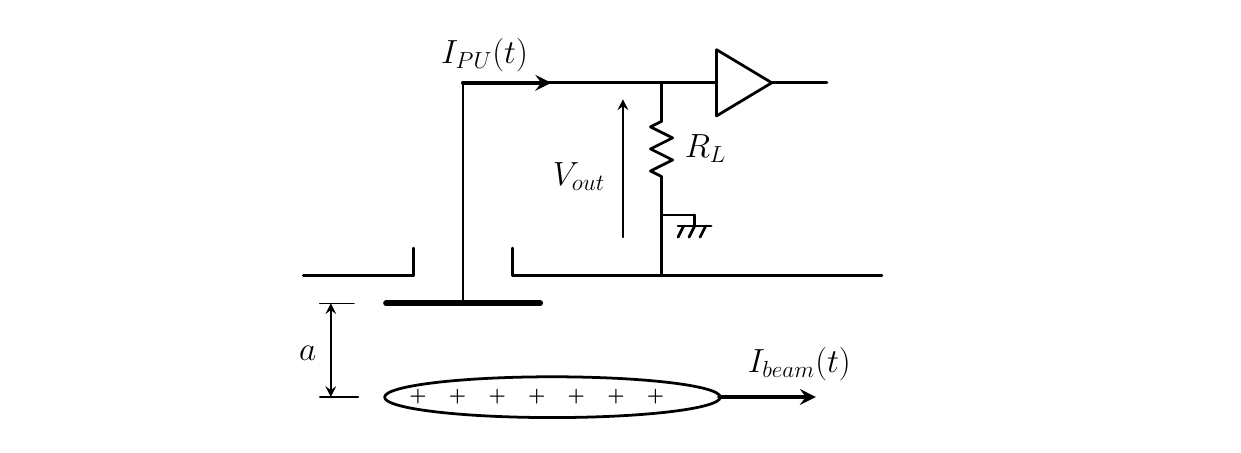
\begin{tikzpicture}[line cap=round,line join=round,>=stealth,x=1cm,y=1cm, scale=0.7, every node/.style={scale=0.7}]

  \clip(-8.5,-2.2) rectangle (13,5);
  \draw [line width=1pt] (3,4)-- (3,3.3);
  \draw [line width=1pt] (3,3.3)-- (2.8,3.2);
  \draw [line width=1pt] (2.8,3.2)-- (3.2,3);
  \draw [line width=1pt] (3.2,3)-- (2.8,2.8);
  \draw [line width=1pt] (2.8,2.8)-- (3.2,2.6);
  \draw [line width=1pt] (3.2,2.6)-- (2.8,2.4);
  \draw [line width=1pt] (3.6,1.6)-- (3.6,1.4);
  \draw [line width=1pt] (3.6,1.4)-- (3.9,1.4);
  \draw [line width=1pt] (3.6,1.4)-- (3.3,1.4);
  \draw [line width=1pt] (3.4,1.4)-- (3.3,1.2);
  \draw [line width=1pt] (3.6,1.4)-- (3.5,1.2);
  \draw [line width=1pt] (3.8,1.4)-- (3.7,1.2);
  \draw [line width=1pt] (3,4)-- (4,4);
  \draw [line width=1pt] (4.,4.6)-- (4.,3.4);
  \draw [line width=1pt] (4.,3.4)-- (5,4);
  \draw [line width=1pt] (5,4)-- (4.,4.6);
  \draw [line width=1pt] (5,4)-- (6,4);
  \draw [line width=1pt] (2.8,2.4)-- (3,2.3);
  \draw [line width=1pt] (3.6,1.6)-- (3,1.6);
  \node[right] at (3.3, 2.8) {\LARGE $R_\text{L}$};

  \draw [rotate around={0:(1.0208488845892716,-1.7039178093053853)},line width=1pt] (1.0208488845892716,-1.7039178093053853) ellipse (3.0448620824106136cm and 0.3699384325291824cm);
  \node[right] at (-1.7,-1.7) {\textbf{+$\quad$+$\quad$+$\quad$+$\quad$+$\quad$+$\quad$+}};

  \draw [->,line width=1.5pt] (4.05,-1.7) -- (5.8,-1.70);
  \draw (5.5, -1.1) node {\parbox{2cm}{\centering \LARGE $I_\text{beam}(t)$ }};

  \draw [line width=.5pt] (-2.5,-1.7)-- (-3.2,-1.7);
  \draw [line width=0.5pt] (-3.2,0)-- (-2.58,0);
  \draw [->,line width=.7pt] (-3,-0.4) -- (-3,-1.7);
  \draw [->,line width=.7pt] (-3,-0.4) -- (-3,0);
  \node[right] at (-3.7,-0.9) {\LARGE $a$};

  \draw [->,line width=.7pt] (2.3,1.2) -- (2.3,3.7);
  \node[left] at (2.1,2.3) {\LARGE $V_\text{out}$};

  \draw [->,line width=1.5pt] (-0.6, 4) -- (1, 4);
  \node[left] at (.7, 4.5) {\LARGE $I_\text{PU}(t)$};


  \draw [line width=1pt] (-0.6,4)-- (3,4);
  \draw [line width=1pt] (3,2.3)-- (3,1.6);
  \draw [line width=1pt] (0.3,1)-- (0.3,0.5);
  \draw [line width=1pt] (0.3,0.5)-- (7,0.5);
  \draw [line width=1pt] (3,1.6)-- (3,0.5);
  \draw [line width=1pt] (-1.5,1)-- (-1.5,0.5);
  \draw [line width=1pt] (-1.5,0.5)-- (-3.5,0.5);
  \draw [line width=2pt] (-2,-0)-- (0.8,-0);
  \draw [line width=1pt] (-0.6,4)-- (-0.6,0);

\end{tikzpicture}

\caption{Schematic representation of the beam interaction with a button BPM.}
\label{fig:button}
\end{figure}

Considering a button with an area $A$ and at a distance $a$ away from the beam, the induced current is~\cite{Forck:CAS}:
\begin{equation}
I_\text{PU} \equiv - \frac{dQ_\text{PU}}{dt} = \frac{A}{2\pi a l} I_\text{beam}(t) = \frac{A}{2\pi a l} \frac{dQ_\text{beam}(t)}{dt}
\end{equation}
where $l$ is the button length. The derivative of the beam charge can be rewritten as
\begin{equation}
\frac{dQ_\text{beam}(t)}{dt} = \frac{l}{\beta c} \frac{dI_\text{beam}(t)}{dt} = \frac{l}{\beta c} I_\text{beam} (\omega),
\end{equation}
where $I_\text{beam}(\omega)$ is the Fourier transform of the beam current, $\beta$ the relativistic velocity and $c$ the speed of light.
Finally, the output voltage can be written 
\begin{equation}
V_{out}(\omega) = Z_t(\beta, \omega) \, I_\text{beam}(\omega),
\end{equation}
where $Z_t$ is defined as the transverse impedance of the BPM. This expression indicates that the signal produced by a BPM is a convolution of its transverse impedance and the beam spectrum. It is fundamental to note that for relativistic beams the transverse impedance depends, to a first approximation, only on the BPM's electric and geometric characteristics. Conversely, the beam spectrum is purely related to the beam physics and it is virtually independent of the instrument design.

The equivalent circuit for an electrostatic button is a current source that produces a portion of $I_\text{beam}(t)$ depending on the button area and the beam distance. The induced current is discharged through the shunt resistor $R_\text{L}$ and the capacitance between the button and the vacuum pipe. Since the impedance is defiend as $Z^{-1} = R^{-1} + i\omega C$, the button voltage becomes
\begin{equation}
V_\text{out}(\omega) = \frac{R_\text{L}}{1+i\omega R_\text{L} C} I_\text{PU}(\omega) = \frac{1}{\beta c} \frac{A}{2\pi a} \frac{R_\text{L}}{1+i\omega R_\text{L} C} I_\text{beam}(\omega) = \Gamma \frac{1}{a} I_\text{beam}(\omega)
\end{equation}
where $\Gamma$ is a term that depends on the geometrical and electrical characteristics of the BPM. The magnituide of the generated signal is inversely proportional to the distance from the beam.

Let us now consider two identical buttons at opposite positions in the beampipe: the buttons $R$ and $L$. The voltage induced by the beam is:
\begin{equation}
V_{R,im}(\omega) = \Gamma \frac{1}{a_R} I_{beam}(\omega)
\end{equation}
\begin{equation}
V_{L,im}(\omega) = \Gamma \frac{1}{a_L} I_{beam}(\omega)
\end{equation}
The two $\Gamma$ factors are identical as they are calculated for identical geometries. The output signals of the two buttons will vary depending on the distances $a_R$ and $a_L$ from the beam. In order to reconstruct the beam position, the $\Delta$ quantity is calculated, defined as the difference of the electrode signals
\begin{equation}
\Delta = V_{R,im} - V_{L,im}(\omega) = \left( \frac{1}{a_R} - \frac{1}{a_L}  \right) \Gamma I_{beam}(\omega)
\end{equation}
This can be made independent of the beam intensity $I_\text{beam}$ and the $\Gamma$ factor by dividing it by the sum of the electrode signals
\begin{equation}
\Sigma = V_{R,im} + V_{L,im}(\omega) = \left( \frac{1}{a_R} + \frac{1}{a_L}  \right) \Gamma I_{beam}(\omega)
\end{equation}
to obtain the $\Delta/\Sigma$ quantity, that is normally used to characterise a BPM response. This has the advantage of being independent of the beam intensity and the button geometry. In fact, the analytical expression is uniquely dependent on the beam position:
\begin{equation}
\frac{\Delta}{\Sigma} = \left( \frac{1}{a_R} - \frac{1}{a_L}  \right) / \left( \frac{1}{a_R} + \frac{1}{a_L}  \right) = \frac{a_L - a_R}{a_L + a_R}\label{eq:delta_sigma}
\end{equation}



\subsection[Effect of multiple beams]{Effect of multiple beams}

The electrostatic BPM response is more complicated when it simultaneously measures two particle bunches with different lengths. Let us consider an electron beam ($e$) and a proton beam ($p$), each of them with Gaussian shape, composed of $N_e$ and $N_p$ particles and with 1-$\sigma$ bunch length of $\sigma_e$ and $\sigma_p$, respectively. The response of the $R$ button is now determined by a superposition of two components:
\begin{equation}
V_{R}(\omega) = \Gamma \frac{1}{a_{R,e}} I_{beam, e}(\omega) +  \Gamma \frac{1}{a_{R,p}} I_{beam, p}(\omega)
\end{equation}
where the terms $a_{R,e}$ and $a_{R,p}$ denote the respective distances of each beam from the button.

Equation~\ref{eq:delta_sigma} becomes dependent not only on the position of both beams, but also on their relative intensities:
\begin{equation}
\frac{\Delta}{\Sigma} = \frac{
\frac{I_{beam,e}(\omega)}{I_{beam,p}(\omega)} \left(\frac{a_{L,e} - a_{R,e}}{a_{L,e} a_{R,e}}\right) - \left(\frac{a_{L,p} - a_{R,p}}{a_{L,p} a_{R,p}}\right)
}{
\frac{I_{beam,e}(\omega)}{I_{beam,p}(\omega)} \left(\frac{a_{L,e} - a_{R,e}}{a_{L,e} a_{R,e}}\right) + \left(\frac{a_{L,p} - a_{R,p}}{a_{L,p} a_{R,p}}\right)
}\label{eq:delta_sigma2}
\end{equation}

Assuming that both bunches have a longitudinal Gaussian distribution, the beam current can be expressed in the time and frequency domains as
\begin{equation}
I_{beam}(t) = \frac{e N}{\sqrt{2\pi} \sigma} \,\text{exp}\left\{  -\frac{1}{2}\frac{t^2}{\sigma^2}  \right\}\label{eq:gauss_bunch}
\end{equation}
\begin{equation}
I_{beam}(\omega) = \frac{e N}{\sqrt{2\pi}} \,\text{exp}\left\{  -\frac{1}{2} \sigma^2 \omega^2  \right\}
\end{equation}

An interesting case for further development of this work is when one bunch is much longer and more intense than the other. This condition is expressed as $\sigma_e << \sigma_p$ and $N_e << N_p$. Therefore, the expression of the bunch spectra for the two bunches becomes:
\begin{equation}
I_{beam,p}(\omega) = \frac{e N_p}{\sqrt{2\pi}} \,\text{exp}\left\{  -\frac{1}{2} \sigma_p^2 \omega^2  \right\}\label{eq:pPower}
\end{equation}
\begin{equation}
I_{beam,e}(\omega) = \frac{e N_e}{\sqrt{2\pi}} \,\text{exp}\left\{  -\frac{1}{2} \sigma_e^2 \omega^2  \right\} \approx \frac{e N_e}{\sqrt{2\pi}}\label{eq:ePower}
\end{equation}
The approximation of the $e$ beam spectrum holds if $\omega \ll 1/\sigma_e$, i.e. in a frequency region where the wavelength is considerably larger than the bunch length. In this frequency region, the $e$ beam spectral power can be considered constant. Figure~\ref{gauss_bunch} presents the beam current in time and frequency domains, for beams with parameters as in Table~\ref{beam_param_exp:tab}.


\begin{figure}[!b]
\centering
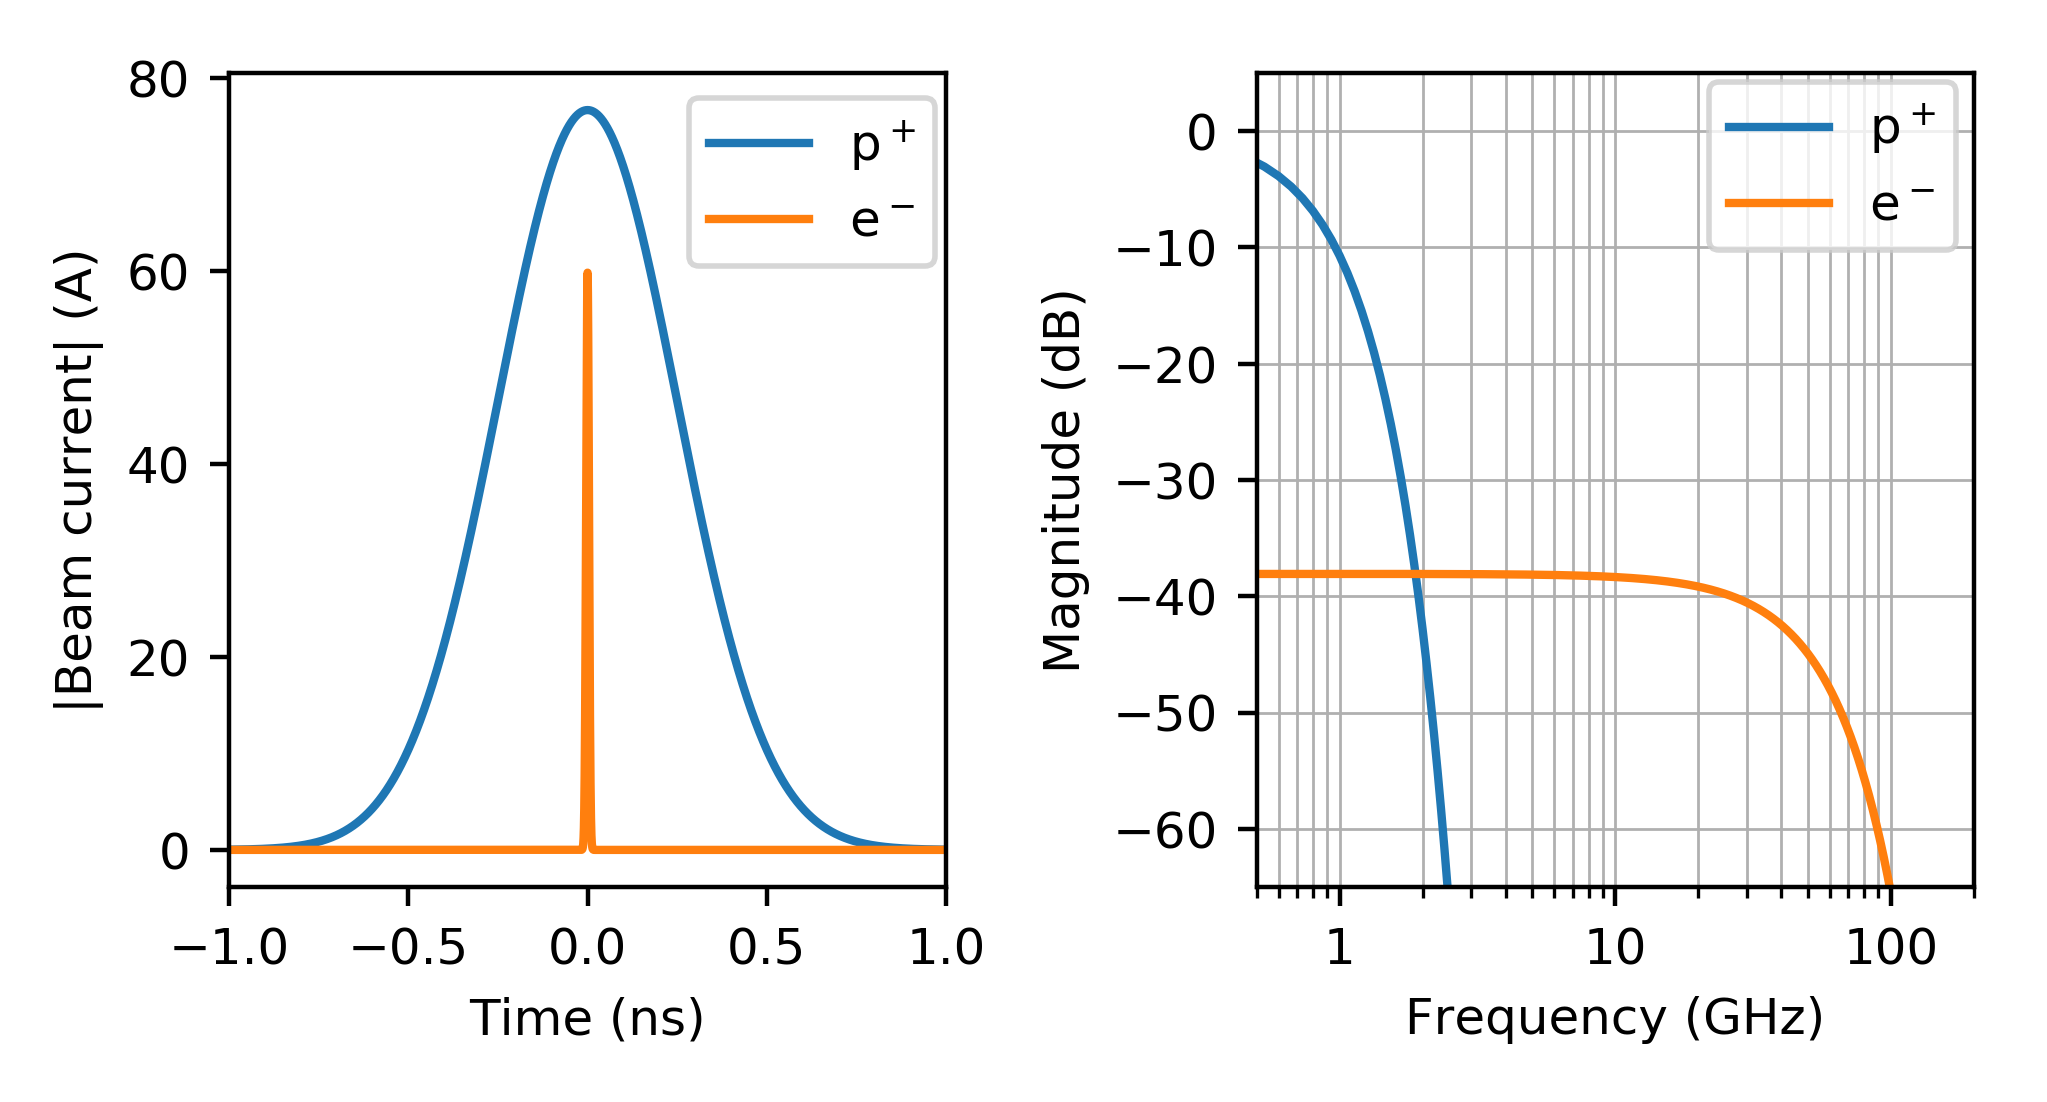
\includegraphics[scale=1., keepaspectratio]{pictures/time_freq_domain}
\caption{Time (on the left) and frequency domain (on the right) comparison of the parameters of the proton and electron bunches reported in Tab.~\ref{beam_param_exp:tab}.}
\label{gauss_bunch}
\end{figure}

The term $I_{beam,e}(\omega)/I_{beam,p}(\omega)$ in Equation~\ref{eq:delta_sigma2} can now be rewritten by means of Equation~\ref{eq:pPower} and \ref{eq:ePower} as
\begin{equation}
\frac{I_{beam,e}(\omega)}{I_{beam,p}(\omega)} = \frac{N_e}{N_p} \,\text{exp}\left\{  \frac{1}{2} \sigma_p^2 \omega^2  \right\}\label{eq:int_ratio}
\end{equation}
This leads to two interesting observations:
\begin{itemize}
\item for $\sigma_p^2 \omega^2 \to 0$: if the detection frequency is not sufficiently high, the exponent in \ref{eq:int_ratio} reduces to 1. From Equation~\ref{eq:delta_sigma2}, the $\Delta/\Sigma$ factor is the sum of the $e$ and $p$ beams contribution, but with the $e$ part attenuated be a factor of $\frac{N_e}{N_p}$. As it has been assumed that $N_e << N_p$, the $\Delta/\Sigma$ response is strongly determined by the $p$ beam position.
\item $\omega >> \sigma_p^{-1}$: if the detection frequency is sufficiently high, the opposite effect will take place. The Equation~\ref{eq:delta_sigma2} terms which depend on the electron-beam position are amplified and the $\Delta/\Sigma$ factor is determined mostly by the electron beam position.
\end{itemize}


In the case of the AWAKE beam parameters reported in Table~\ref{beam_param_exp:tab}, the two beams have the same spectral power at 1.9~GHz, as shown in Fig.~\ref{gauss_bunch}. The approximation in Eq.~\ref{eq:ePower} of constant electron spectral power in this frequency range introduces an error of the order of 0.1\textperthousand, and it is therefore justified.

\begin{table}[h]
  \centering
    \begin{tabular}{l c c c}
    \toprule
    Name  & \multicolumn{2}{c}{Charge} & $\sigma$\\
          & nC & ppb & ps\\
    \midrule
    Proton beam								& $48$	  & $3\times10^{11}$	& 250	\\
    Electron beam							& $0.6$	  & $3.7\times10^{9}$	& 4		\\
    \bottomrule
    \end{tabular}
  \caption{Beam parameters used in AWAKE.} \label{beam_param_exp:tab}
\end{table}





% \subsection[Shorted striplines]{Shorted striplines}

% It is useful to extend these consideration to shorted stripline-type pickups as the AWAKE electron BPMs use this design. Stripline pickups are formed of a metallic strip that is terminated a the two extremities. In the case of shorted striplines, one of the extremities is shorted to the beampipe, while the second one is matched to the output with a $50\,\Omega$ termination impedance. Figure~\ref{fig:shorted_stripline} shows a schematic representation of a shorted stripline. Stripline BPMs present a number of advantages compared to buttons, like larger coverage and so signal intensity, and directionality.

% \begin{figure}[bh]
% \centering
% 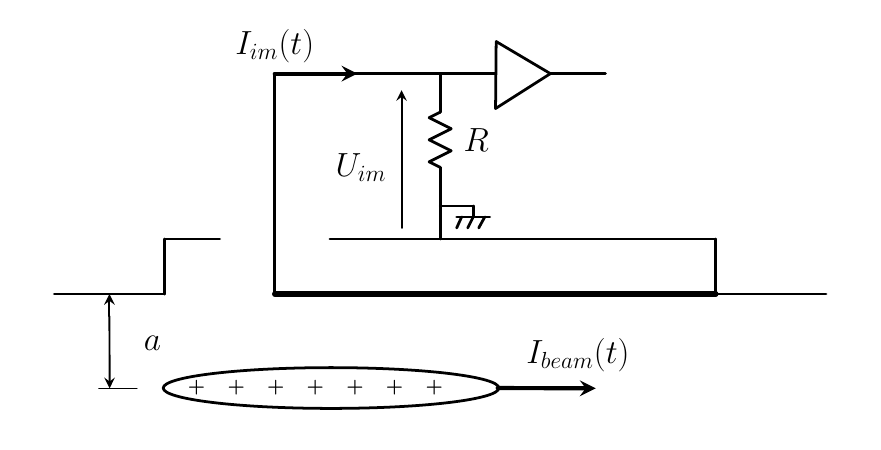
\begin{tikzpicture}[line cap=round,line join=round,>=stealth,x=1cm,y=1cm, scale=0.7, every node/.style={scale=0.7}]
\clip(-4.483337037047517,-2.309172461417361) rectangle (10.480749878095986,4.83380807328732);
\draw [line width=1pt] (-4,0)-- (-2,0);
\draw [line width=1pt] (-2,0)-- (-2,1);
\draw [line width=1pt] (-2,1)-- (-1,1);
\draw [line width=1pt] (1,1)-- (8,1);
\draw [line width=1pt] (8,1)-- (8,0);
\draw [line width=2pt, sharp corners] (8,0)-- (0,0);
\draw [line width=1pt] (8,0)-- (10,0);
\draw [line width=1pt] (0,0)-- (0,4);
\draw [line width=1pt] (0,4)-- (3,4);
\draw [line width=1pt] (3,4)-- (3,3.3);
\draw [line width=1pt] (3,3.3)-- (2.8,3.2);
\draw [line width=1pt] (2.8,3.2)-- (3.2,3);
\draw [line width=1pt] (3.2,3)-- (2.8,2.8);
\draw [line width=1pt] (2.8,2.8)-- (3.2,2.6);
\draw [line width=1pt] (3.2,2.6)-- (2.8,2.4);
\draw [line width=1pt] (3.6,1.6)-- (3.6,1.4);
\draw [line width=1pt] (3.6,1.4)-- (3.9,1.4);
\draw [line width=1pt] (3.6,1.4)-- (3.3,1.4);
\draw [line width=1pt] (3.389508749461253,1.4)-- (3.3,1.2);
\draw [line width=1pt] (3.6,1.4)-- (3.5,1.2);
\draw [line width=1pt] (3.8095747679309224,1.4)-- (3.7,1.2);
\draw [line width=1pt] (3,4)-- (4,4);
\draw [line width=1pt] (4.016612671646594,4.582041781632238)-- (4.005361353434939,3.3668994147734796);
\draw [line width=1pt] (4.005361353434939,3.3668994147734796)-- (5,4);
\draw [line width=1pt] (5,4)-- (4.016612671646594,4.582041781632238);
\draw [line width=1pt] (5,4)-- (6,4);
\draw [line width=1pt] (2.8,2.4)-- (3,2.3);
\draw [line width=1pt] (3,2.3)-- (3,1);
\draw [line width=1pt] (3.6,1.6)-- (3,1.6);
\node[right] at (3.3, 2.8) {\LARGE $R$};


\draw [rotate around={0:(1.0208488845892716,-1.7039178093053853)},line width=1pt] (1.0208488845892716,-1.7039178093053853) ellipse (3.0448620824106136cm and 0.3699384325291824cm);
\node[right] at (-1.7,-1.7) {\textbf{+$\quad$+$\quad$+$\quad$+$\quad$+$\quad$+$\quad$+}};

\draw [->,line width=1.5pt] (4.043154404724465,-1.7039178093053853) -- (5.82375758656814,-1.7098538305482853);
% \node[top] at (5.5, -1.1) {\LARGE $I_\text{beam}(t)$};
\draw (5.5, -1.1) node {\parbox{2cm}{\centering \LARGE $I_\text{beam}(t)$ }};

\draw [line width=.5pt] (-2.5013938519865704,-1.7088902243743347)-- (-3.191514587584385,-1.7088902243743347);
\draw [->,line width=.7pt] (-3,-0.4) -- (-2.9965949905071394,-1.7088902243743345);
\draw [->,line width=.7pt] (-3,-0.4) -- (-3,0);
\node[right] at (-2.5,-0.9) {\LARGE $a$};


\draw [->,line width=.7pt] (2.3,1.2) -- (2.3,3.7);
\node[left] at (2.15,2.3) {\LARGE $U_\text{im}$};

\draw [->,line width=1.5pt] (0, 4) -- (1.5, 4);
% \node[top] at (0, 4.5) {\LARGE $I_\text{im}(t)$};
\draw (0, 4.5) node {\parbox{2cm}{\centering \LARGE $I_\text{im}(t)$ }};

\end{tikzpicture}

% \caption{A simple rappresentation.}
% \label{fig:shorted_stripline}
% \end{figure}

% The properties of striplines are well know as they are widely used as transmission lines in the electronics in the microwave regime \cite{Pozar:MW_engineering}. In shorted striplines, the bunch signal is reflected with opposite polarity at the termination and reaches the output after a delay $\Delta t = 2l/c$, where $l$ is the stripline length and $c$ the speed of light. For the gaussian bunch in Eq.~\ref{eq:gauss_bunch}, the output signal can be expressed as
% \begin{equation}
% U(t) = Z_\text{strip} \frac{\alpha}{4 \pi} \frac{eN}{\sqrt{2\pi}\sigma} \left[ \,\text{exp}\left\{  -\frac{1}{2}\frac{t^2}{\sigma^2}  \right\} - \,\text{exp}\left\{  -\frac{1}{2}\frac{(t-2l/c)^2}{\sigma^2}  \right\}   \right]
% \label{eq:striplines}
% \end{equation}
% where $Z_\text{strip}$ is the stripline impedance \cite{Forck:CAS}.



% The Figures~\ref{stripline_theor1} and \ref{stripline_theor2} show the beam current and its reflection in the time and frequency domain for an ideal stripline. The beam parameters in Table~\ref{beam_param_exp:tab} are used. In the plots, it is depicted the quantity in Eq.~\ref{eq:striplines} neglecting the constant factor $Z_\text{strip} \frac{\alpha}{4 \pi}$.
% In the frequency domain, the presence of the reflections causes the appearance of notches in the spectrum. The notches position does not depend on the beam parameters, but on the stripline length only. The frequency at which the detection works has therefore to be chosen in order to maximise the signal output power.



% \begin{figure}[h]
% \centering
% \subfigure[Time domain response]
%   {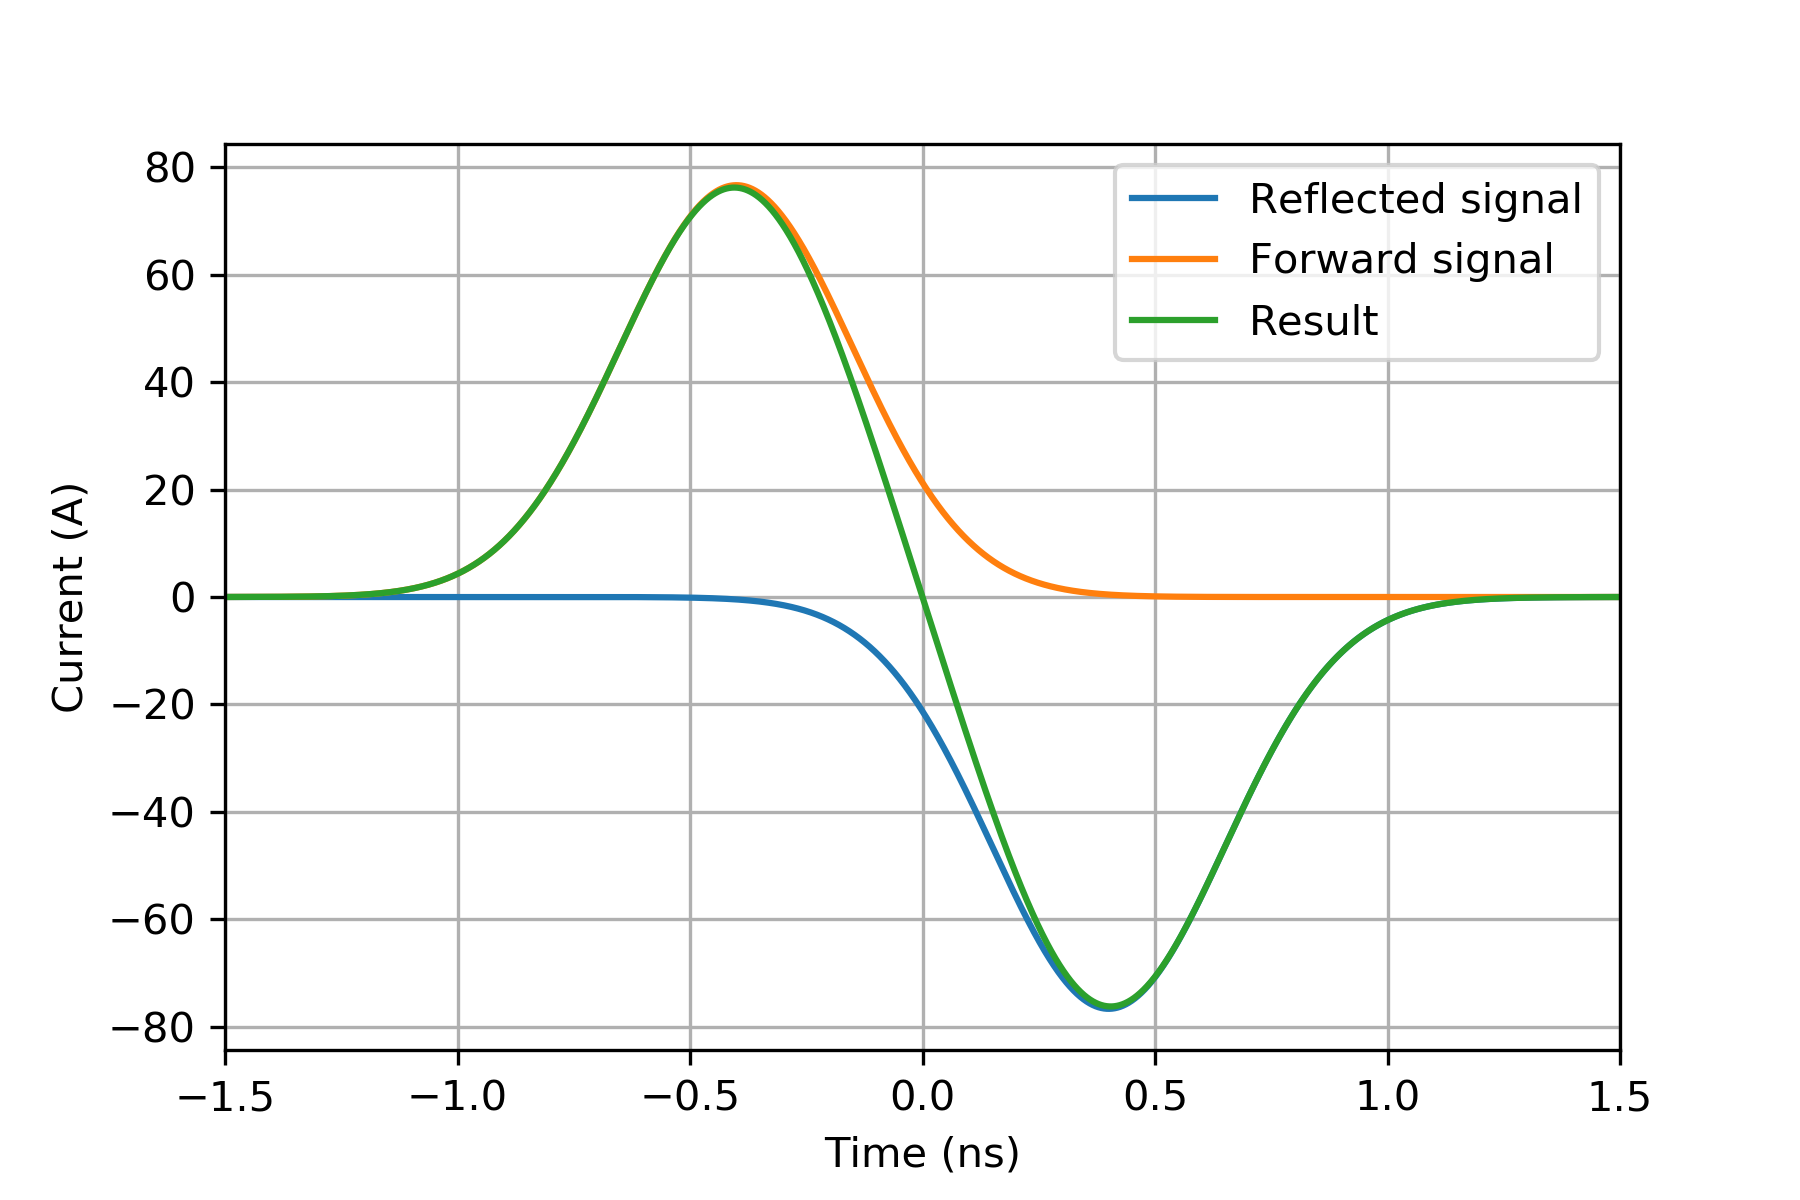
\includegraphics[width=6.5cm,height=5cm]{pictures/stripline_p_signals}}
% \hspace{3mm}
% \subfigure[Frequency domain response]
%   {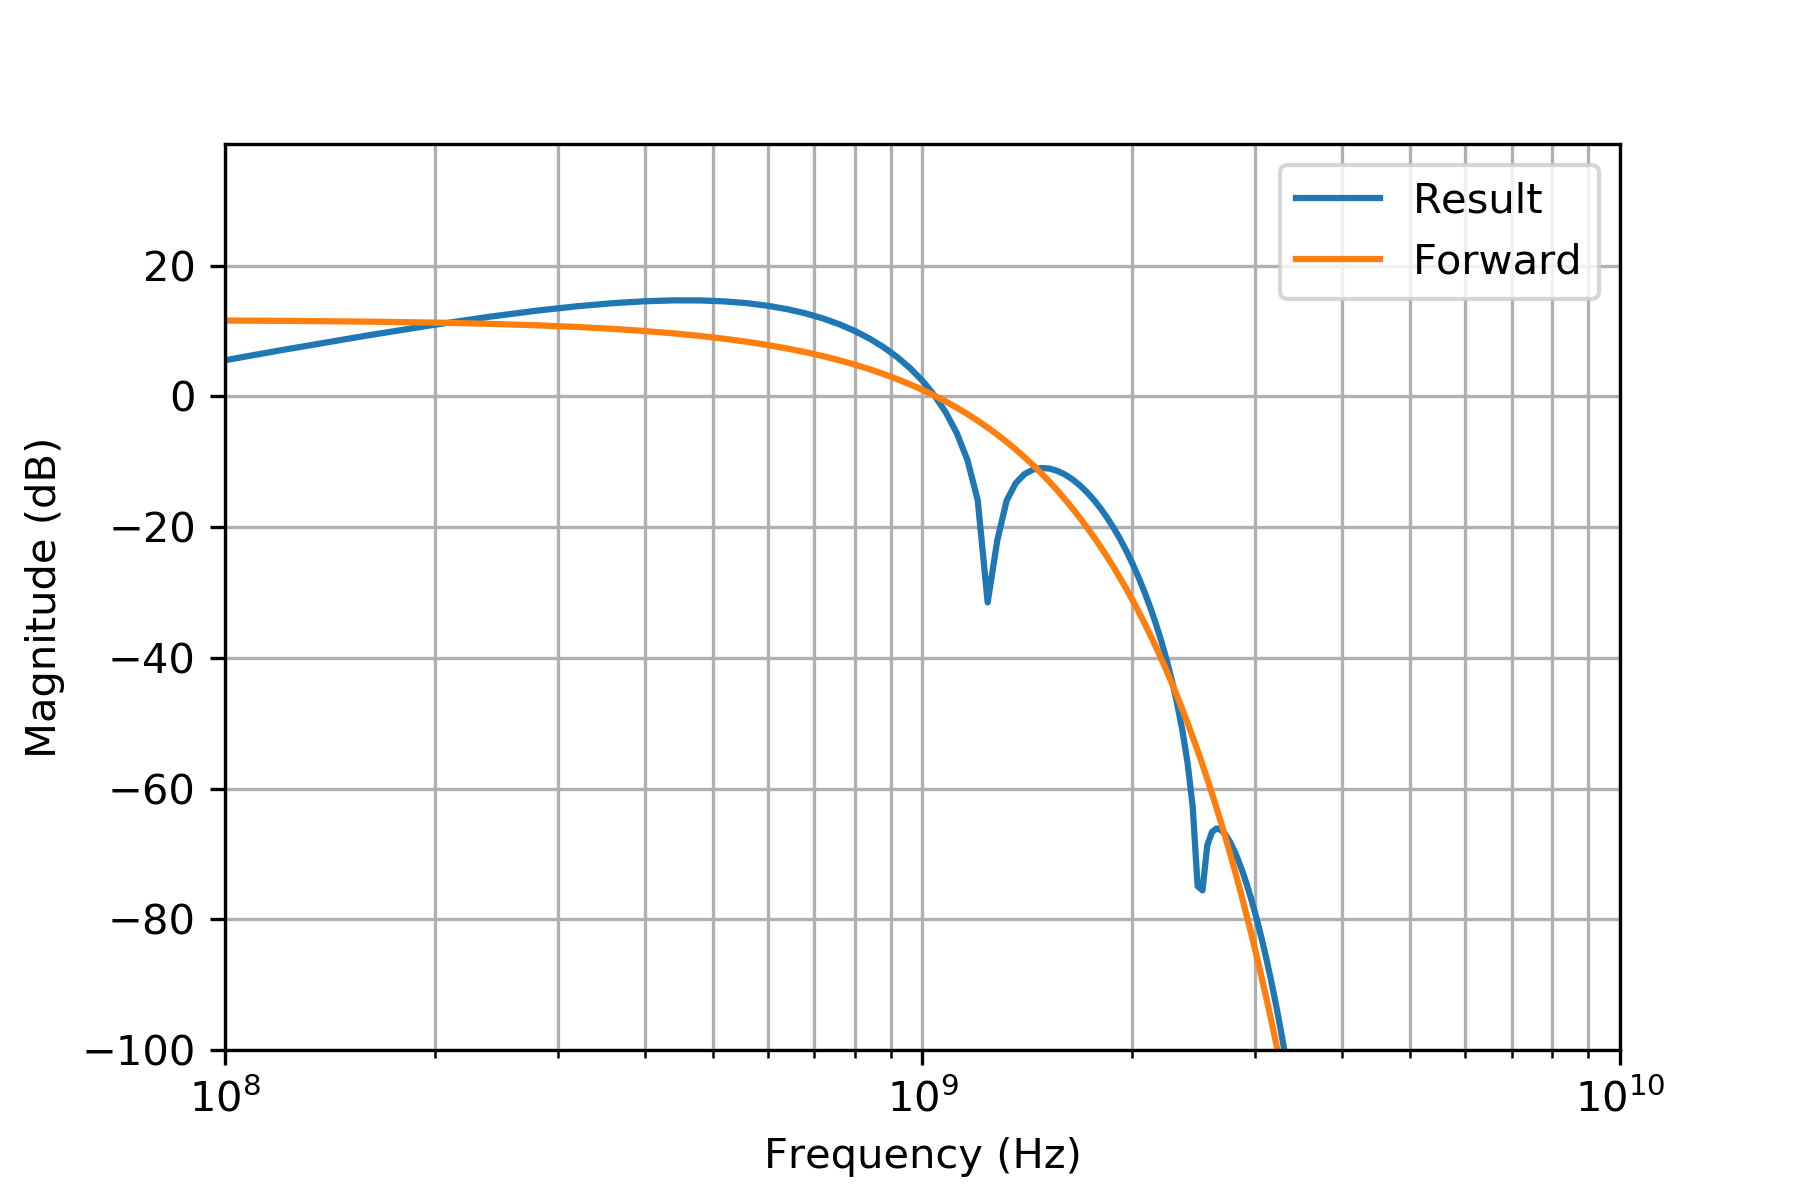
\includegraphics[width=6.5cm,height=5cm]{pictures/stripline_p_freqs}}
% \caption{Shorted stripline response for a 4.7~nC, 250~ps-$\sigma$ beam. }
% \label{stripline_theor1}
% \end{figure}

% \begin{figure}[h]
% \centering
% \subfigure[Time domain response]
%   {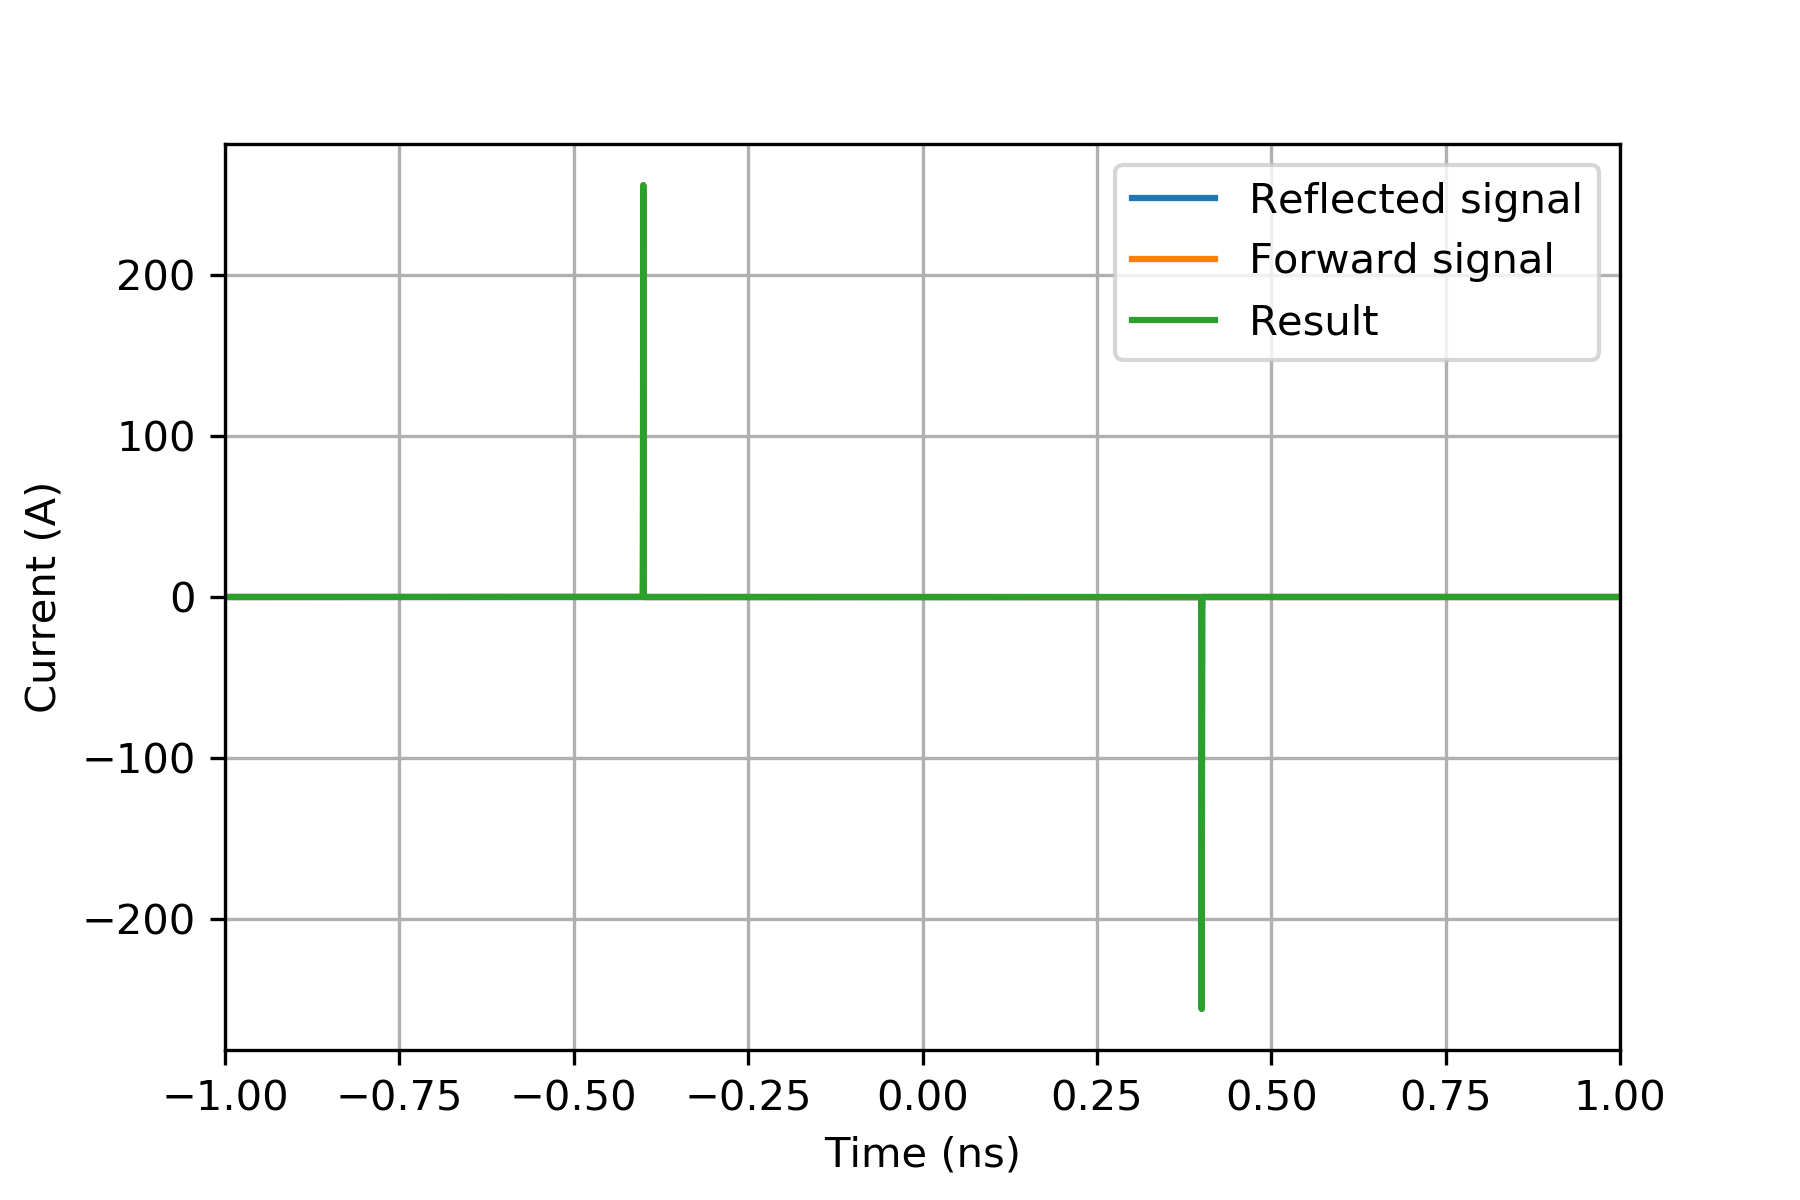
\includegraphics[width=6.5cm, height=5cm]{pictures/stripline_e_signals}}
% \hspace{3mm}
% \subfigure[Frequency domain response]
%   {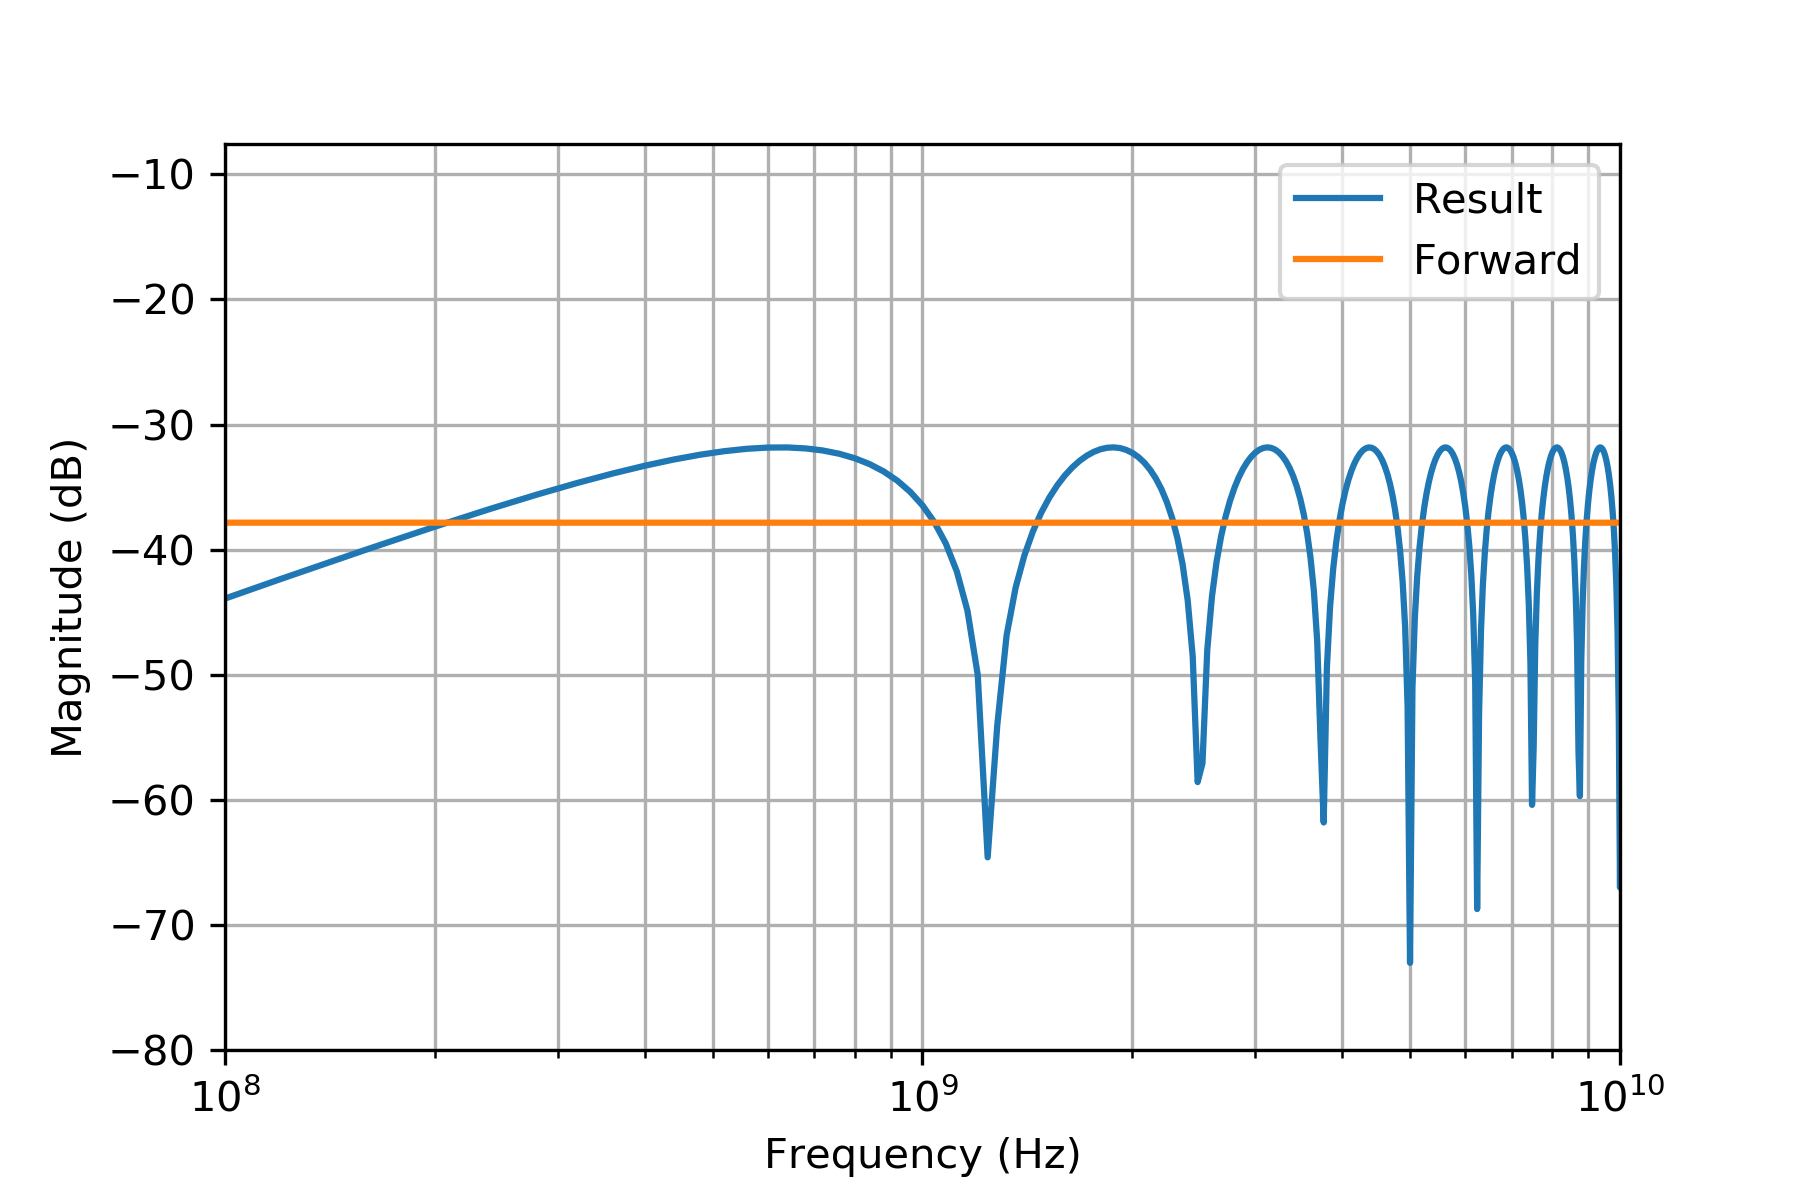
\includegraphics[width=6.5cm, height=5cm]{pictures/stripline_e_freqs}}
% \caption{Shorted stripline response for a 0.6~nC, 1~ps-$\sigma$ beam. }
% \label{stripline_theor2}
% \end{figure}


\section[Design parameter constraints]{Design parameter constraints}

The constraints in designing beam instrumentation for the AWAKE experiment are listed in Table.~\ref{awake_all_params:tab}. They are set by both the beam parameters, and the beampipe dimensions.

\begin{table}[t]
  \centering
    \begin{tabular}{l c c}
    \toprule
    Parameter & p$^+$ beam & e$^-$ beam\\
    \midrule
    Beampipe diameter & \multicolumn{2}{c}{$60$ mm}\\
    \hline \rule{0pt}{2.5ex}
    Charge 	    & $48$ nC	&  $100-600$ pC \\
    Length      & $250$ ps  &   $1-4$ ps\\
    Energy      & $400$ GeV   &   $16-20$ MeV\\
    \bottomrule
    \end{tabular}
  \caption{AWAKE parameters for this study.} \label{awake_all_params:tab}
\end{table}

A key parameter for the design is the rather large beampipe aperture of 60~mm which constitutes an additional complication for a beam position monitoring system working at high frequencies. The beampipe itself acts as a circular waveguide, propagating the electromagnetic waves with frequencies above the cutoff frequency of
\begin{equation}
f_c = \frac{1.8412 \,c}{2 \pi r} = 2.93\text{ GHz}
\end{equation}
where $r$ is the waveguide radius and $c$ the speed of light~\cite{Jackson:490457}. Unwanted electromagnetic radiation is expected to be generated by the beam passage through the vacuum chamber discontinuities, and will propagate along the beampipe, with some fraction of it potentially coupling to the BPM system and resulting in an unwanted spurious signal. In the case of AWAKE, this phenomenon is particularly likely to occur as several metres of the beamline near the plasma cell contain a large number of insertions and diagnostic devices. Therefore, a pickup operating above the beampipe cutoff frequency  will not only produce a signal contaminated by the unwanted wakefields, but also the amount of spurious signal will depend on its exact installation location.

Another fundamental design constraint is given by the large charge ratio between the proton and electron beams. For the moment, both beams are considered to have a Gaussian longitudinal charge distribution. The implications of a different shape of the proton beam are discussed in Section~\ref{sec:proton_shape}. 
The power of the most intense electron beam, with a charge of 600 pC, is 38~dB lower at DC than that of the proton beam, as shown in Fig.~\ref{spectrum_run2}. The electron bunch charge of 100~pC corresponds to an additional decrease of 15.5~dB of the spectral power. Under these conditions, the point at which the electron and proton beams feature the same spectral power moves between 1.9~GHz and 2.2~GHz. As discussed previously, successful detection of the electron beam has to be carried out at frequencies higher than these, to reduce the contribution of the proton beam to the signal. 


\begin{figure}[!h]
\centering
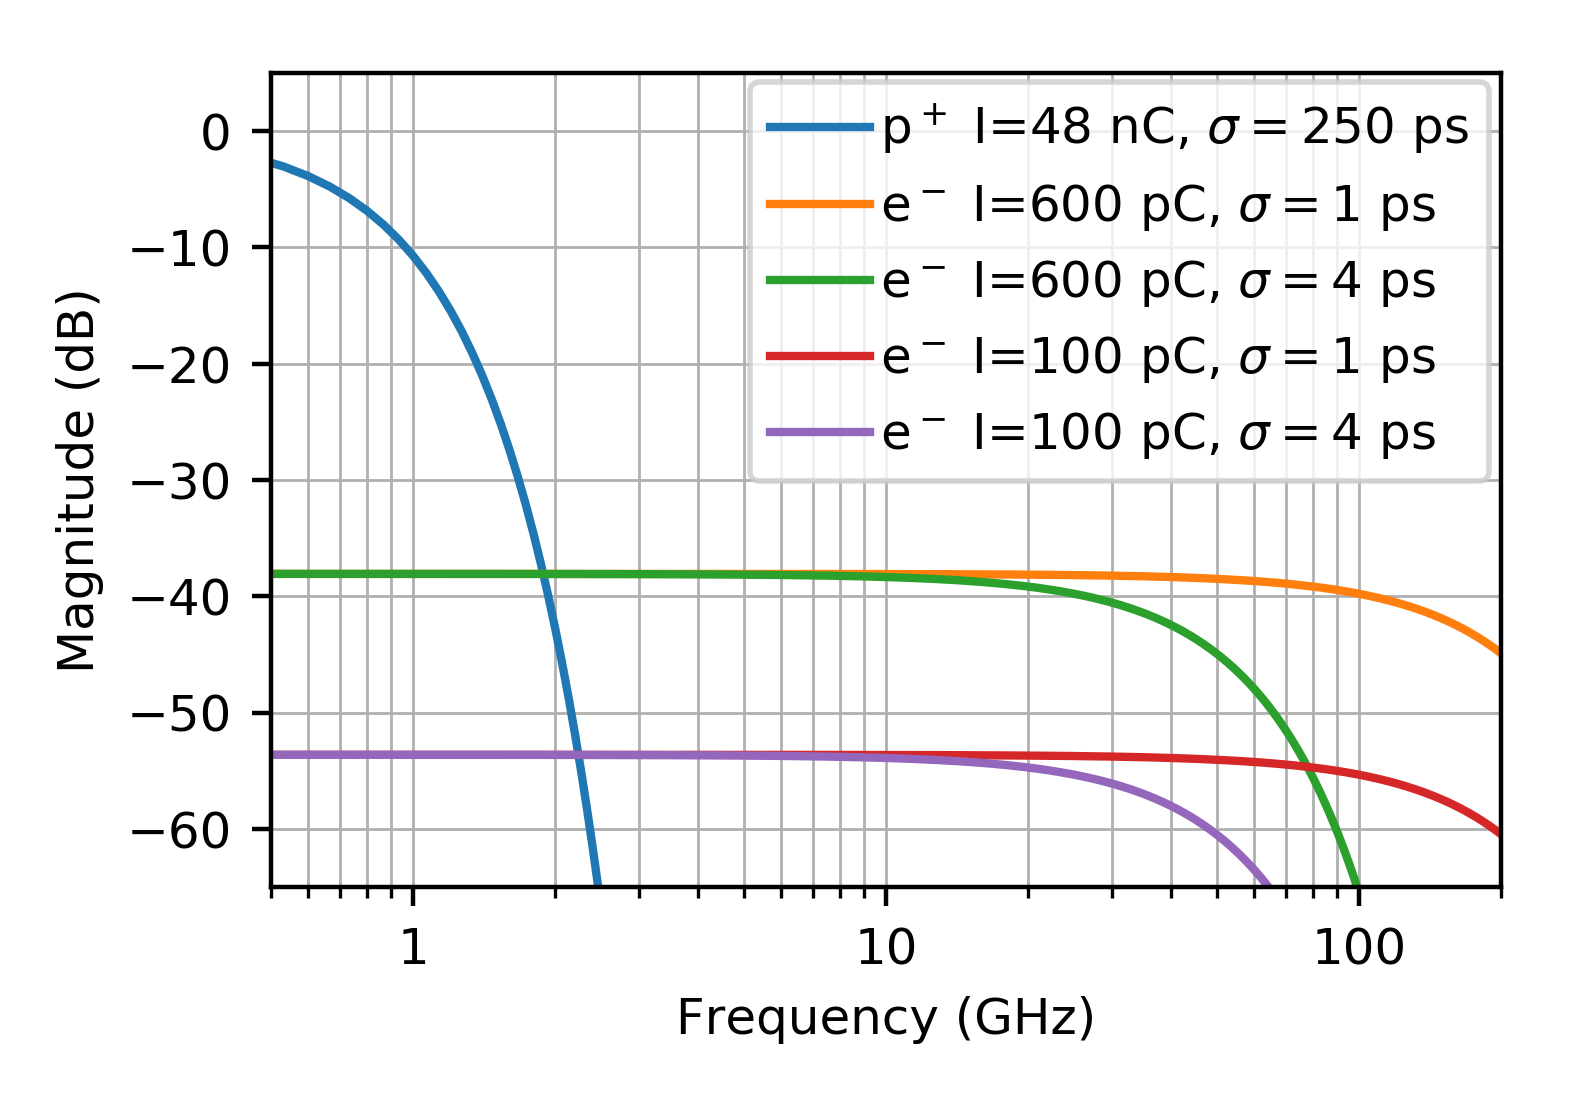
\includegraphics[scale=1.1, keepaspectratio]{pictures/ideal}
\caption{Beam spectral power as function of frequency for AWAKE experiment assuming Gaussian beams.}
\label{spectrum_run2}
\end{figure}







\newpage




\section[Proton beam spectrum measurement]{Proton beam spectrum measurement}\label{sec:proton_shape}

The preceding discussion shows that for the AWAKE beam parameters, a frequency range in which the signal generated by the electron beam is stronger than the proton signal has to be determined. Assuming Gaussian longitudinal charge distributions for both beams, this frequency is above 1.9 or 2.2~GHz, depending on the operational scenario.

A fundamental question to be answered is whether the proton bunch longitudinal distribution extracted from the SPS can be approximated by a Gaussian curve. A non-Gaussian beam shape could include stronger components at high frequency, and therefore increase the frequency which both beams have the same power. Therefore, the correct determination of the proton bunch spectrum is crucial for selecting the operating frequency of an electron beam position monitoring system.

Conversely, this issue does not apply to the electron bunch, as due to its very short duration, the spectral power will remain constant up to tens of GHz. At even higher frequencies, the electron spectrum will drop similarly. Therefore, for the purpose of this study, the electron beam is assumed Gaussian. 

Selecting the electron BPM system working frequency has a large impact on the possible technical solutions that can be exploited to carry out the measurement. Although it is possible to build a pickup using conventional coaxial components working at very high frequencies, this becomes increasingly difficult above around 20 GHz.

The proton beam at AWAKE is produced  in the CERN accelerator complex, using a modified version of an LHC-type beam with higher intensity~\cite{Papaphilippou:2031187, Timko:1595512}. The proton bunch is accelerated up to 400~GeV in the SPS, and then it is adiabatically rotated in  longitudinal phase space in order to shorten its length. The beam is stored in the SPS for an arbitrary period of time, waiting for the synchronisation with the AWAKE laser system. Therefore, after the rotation, the bunch is extracted each time at a different synchrotron phase and the resulting beam longitudinal profule varies shot-by-shot. This effect is worsened if the bunch has an internal sub-structure. Sources of longitudinal bunch profile imperfections can be e.g. energy and phase mismatch in the accelerator, and an imperfect extraction trajectory that causes the beam to scrape on the extraction septum aperture~\cite{handbook_acc_phys}.

It is not possible to study the beam profile variation in the SPS before the extraction as the only suitable instrument installed in the SPS is the Wall Current Monitor \cite{Papotti:private-comm} but its bandwidth does not exceed 2~GHz~\cite{Bohl:1164165} which is not sufficient to resolve the profiles in the frequency range interesting for this study. The AWAKE beamline is better equipped for such a measurement, as it uses longitudinal beam diagnostics to observe the proton bunch self-modulation in plasma \cite{PhysRevLett.122.054802}.




\subsection[Longitudinal beam profile measurement]{Longitudinal beam profile measurement} \label{sec:p_temporal_profile}

A number of scintillation and Optical Transition Radiation (OTR) screens are installed in the AWAKE beamline both up- and down-stream of the plasma cell~\cite{Mazzoni:2017gek}. They are generally used for beam emittance measurements. The OTR screens, although presenting a modest light yield compared with the scintillation screens, can be also used to sample the bunch longitudinal structure and measure the bunch length, due to their intrinsically fast response. 

OTR is emitted when a particle traverses a material discontinuity, generating photons due to the different permittivities in the forward and backward directions~\cite{Ginzburg:306834}. To measure the temporal distribution of the proton bunch, an OTR screen is placed 3.5~m downstream from the plasma-cell exit~\cite{Bachmann_streak}. A schematic representation of the setup is shown in Fig.~\ref{fig:OTR_setup}. The screen is made of a 280~$\mu\text{m}$ thick silicon wafer coated with 1~$\mu\text{m}$ aluminum. The backward-emitted transition radiation is sent through an optical line to a streak camera. Before entering the streak camera, the light is filtered using a bandpass filter with a central wavelength of 450~nm and a passband of 50~nm. The filter limits the optical dispersion effects from the optical transfer line and levels off the energy of the photons arriving at the streak camera photocathode, preventing resolution loss due to chromatic effects. 


\begin{figure}[!t]
\centering
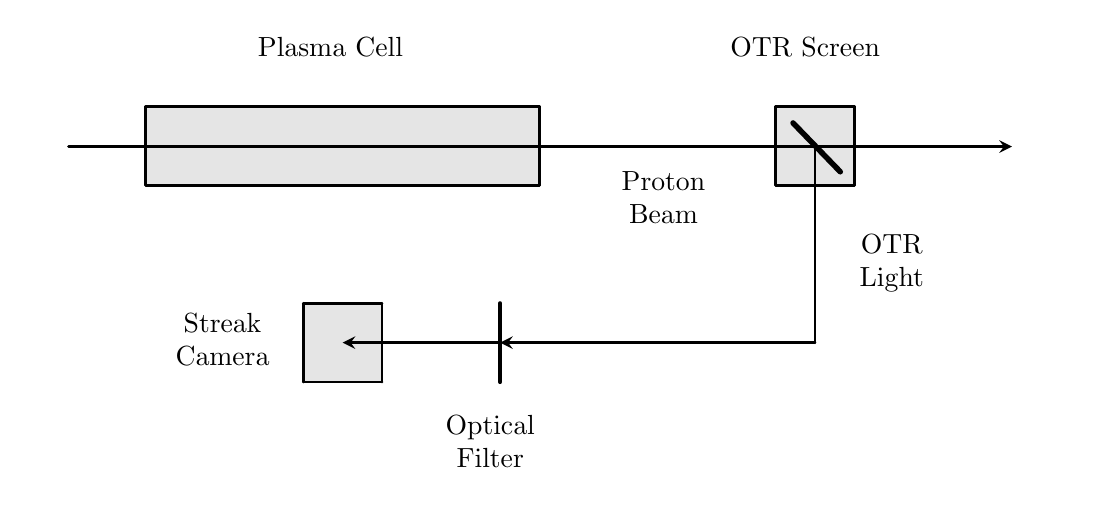
\begin{tikzpicture}[line cap=round,line join=round,>=stealth,x=1cm,y=1cm]

\clip(-1.5,-4) rectangle (12,2);


\fill[line width=1pt,color=black,fill=black,fill opacity=0.1] (0,0) -- (0,1) -- (5,1) -- (5,0) -- cycle;
\fill[line width=1pt,color=black,fill=black,fill opacity=0.1] (8,1) -- (9,1) -- (9,0) -- (8,0) -- cycle;
\fill[line width=1pt,color=black,fill=black,fill opacity=0.1] (2,-1.5) -- (3,-1.5) -- (3,-2.5) -- (2,-2.5) -- cycle;

\draw [line width=1pt,color=black] (0,0)-- (0,1);
\draw [line width=1pt,color=black] (0,1)-- (5,1);
\draw [line width=1pt,color=black] (5,1)-- (5,0);
\draw [line width=1pt,color=black] (5,0)-- (0,0);
\draw [->,line width=1pt] (-0.98,0.49) -- (11,0.49);
\draw [line width=1pt,color=black] (8,1)-- (9,1);
\draw [line width=1pt,color=black] (9,1)-- (9,0);
\draw [line width=1pt,color=black] (9,0)-- (8,0);
\draw [line width=1pt,color=black] (8,0)-- (8,1);
\draw [line width=2pt] (8.22,0.79)-- (8.82,0.17);
\draw [line width=1pt] (8.5,0.5)-- (8.5,-2);

\draw [->,line width=1pt] (8.5,-2) -- (4.5,-2);
\draw [line width=1.5pt] (4.5,-1.5)-- (4.5,-2.5);

\draw [->,line width=1pt] (4.5,-2) -- (2.5,-2);

\draw [line width=1pt,color=black] (2,-1.5)-- (3,-1.5);
\draw [line width=1pt,color=black] (3,-1.5)-- (3,-2.5);
\draw [line width=1pt,color=black] (3,-2.5)-- (2,-2.5);
\draw [line width=1pt,color=black] (2,-2.5)-- (2,-1.5);

\draw (1.3, 2) node[anchor=north west] {Plasma Cell};
\draw (7.3, 2) node[anchor=north west] {\parbox{2.5 cm}{OTR Screen}};
\draw (5.2, 0.3) node[anchor=north west] {\parbox{2.5 cm}{\centering Proton\\ Beam}};
\draw (8.1,-0.5) node[anchor=north west] {\parbox{2.5 cm}{\centering OTR \\ Light}};
\draw (3.0,-2.8) node[anchor=north west] {\parbox{2.5 cm}{\centering Optical \\ Filter}};
\draw (-0.4,-1.5) node[anchor=north west] {\parbox{2.5 cm}{\centering Streak\\Camera}};
\end{tikzpicture}

\caption{Schematic representation of the setup for longitudinal profile measurement.}
\label{fig:OTR_setup}
\end{figure}


A streak camera is the only camera type that is capable of measuring the temporal profile of a light pulse while sacrificing the information on one of the two spatial directions. The principle of operation of a streak camera is shown in Fig.~\ref{fig:streak_hama}. The incident light pulse hits a photocathode after passing through a narrow slit, and gets converted to an electron beam with the same temporal structure. The produced electron beam is accelerated by a static potential difference, and then passes between two deflection plates with a time-varying potential difference applied between them. The potential difference determines the electron bunch tilt, as the head and the tail of the bunch are subjected to a different potential. This process maps the longitudinal bunch structure into a transverse profile. The electron bunch is then amplified by a MicroChannel Plate (MCP) and reaches a phosphor screen where the electrons are converted back into light. Finally, the light is recorded by a camera.

\begin{figure}[!t]
\centering
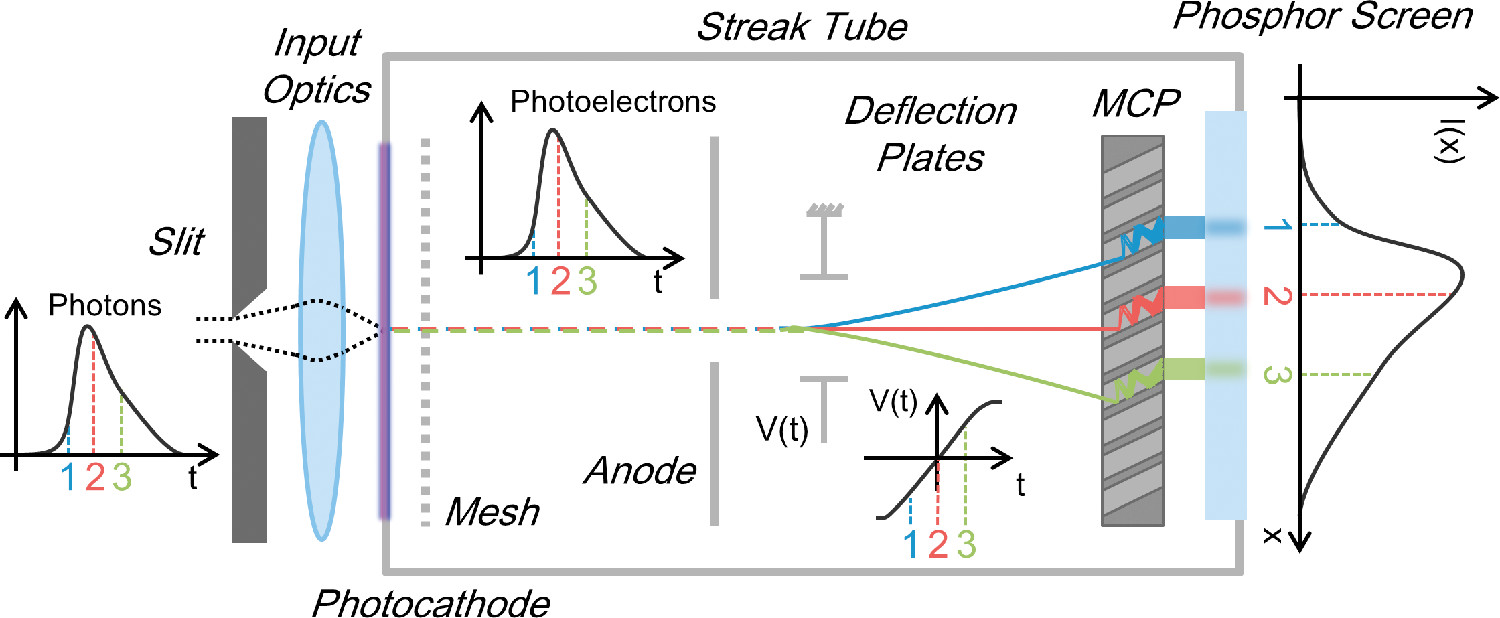
\includegraphics[width=13.5cm, keepaspectratio]{pictures/streak_AIP_paper}
\caption{ Schematic representation of the streak camera principle of operation \cite{doi:10.1063/1.4930122}.}
\label{fig:streak_hama}
\end{figure}

As outlined above, a streak camera measurement presents a high degree of complexity. In fact, the temporal resolution of a streak camera is intrinsically limited by the incident photon flux, and so the produced electron current which is proportional to the input light intensity. With large enough electron current, a strong space-charge force will increase the beam size, resulting in a dilated temporal profile of the camera output pulse. Hence, streak cameras are usually operated with limited input light and a sufficient output signal is produced via frame stacking. However, such a technique cannot be used for precise beam-profile measurements and each output profile has to be considered separately. Nonetheless, accurate estimation of the high-frequency components in the measured profile is not trivial since each single profile is polluted by the camera noise. 

A Hamamatsu streak camera with ps resolution \cite{hama_streak} is installed in the AWAKE experiment and is used to measure primarily the effect of the plasma wakefields on the proton beam \cite{PhysRevLett.122.054802, Bachmann_streak}. A longitudinal profile of an undulated proton bunch was measured using a time window of 1~ns, a slit width of 20~$\mu\text{m}$ and MCP gain of 40. Figure~\ref{fig:streak_image} presents a typical proton bunch streak camera image. 
\begin{figure}[!t]
\centering
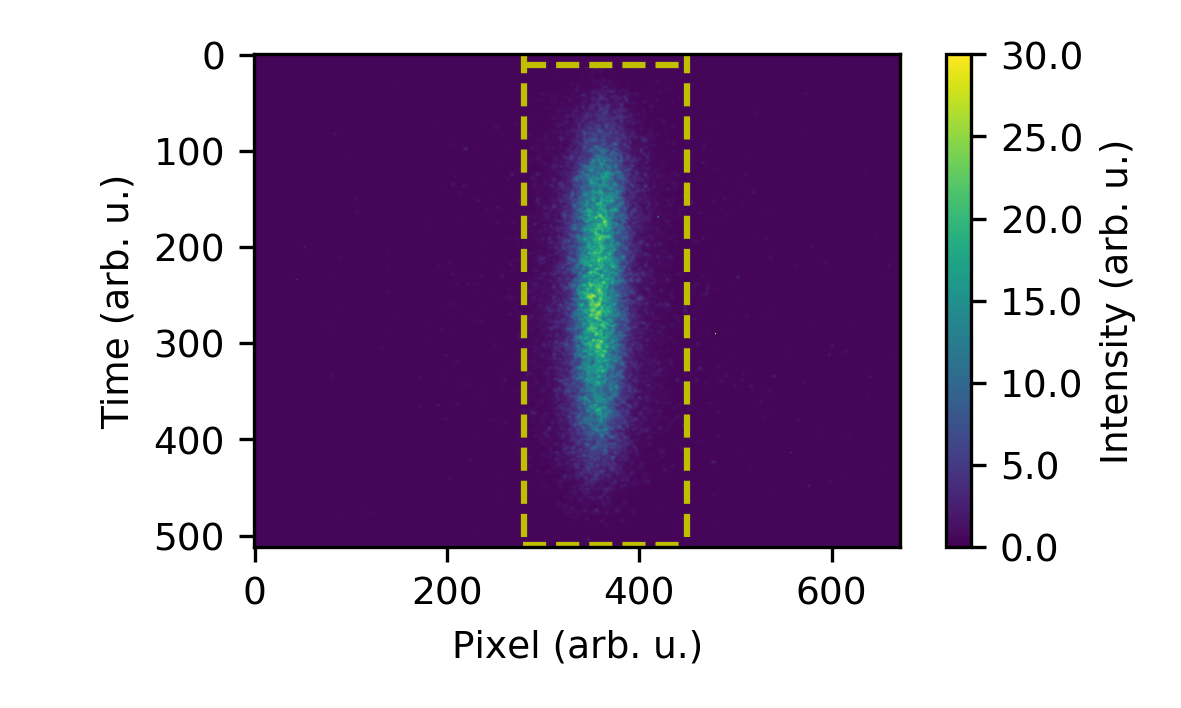
\includegraphics[scale=1.15, keepaspectratio]{pictures/streak_image_thesis}
\caption{A streak camera image of the OTR light for an AWAKE proton bunch of $2.1\times10^{11}$ protons. The vertical axis is time with one pixel being 2.2~ps. The horizontal axis is one of the transverse dimensions of the OTR light beam. The dashed yellow rectangle indicates the region of interest for beam profile calculation.}
\label{fig:streak_image}
\end{figure}
The beam profile is obtained by integrating the pixel intensity over the rows of the sensor matrix in the region of interest (ROI) to reduce the noise resulting from the dark areas. The pixel intensities are compensated to remove the effect of non-linear streak voltage which is recorded for each frame. Once a beam profile is obtained it is zero-padded and its baseline is removed. The plots in the left column of Fig.~\ref{fig:streak_profiles} show three examples of recorded longitudinal beam profiles. A Gaussian fit of each profile is also reported for comparison. Although some intensity dependent noise is expected from the used streak camera, the proton bunch presents consistent features clearly deviating from an idealistic Gaussian profile. In particular, the sharp edges at the beginning and at the end of the profiles cannot be attributed to the measurement noise.

A frequency domain representation of the measured profiles is presented in the right column of Fig.~\ref{fig:streak_profiles} and compared to that of the fitted Gaussian curve. High resolution of the Fourier transform is achieved through zero-padding of the time domain profile, elongating the considered time window by a factor of 32.8. The zero padding consists of artificially elongating the profile tails, adding measurement points of zero value before and after the measured signal. In this case, this process does not alter the physical content of the signal (which has the form of a narrow pulse). This elongation of the profile in time domain provokes a finer binning of the spectrum in the frequency domain, as for the Discrete Fourier Transform (DFT) the binning is
$ \Delta f = 1 / T_s$
where $\Delta f$ is the frequency binning and $T_s$ is the signal length in time domain \cite{DSP-guide}. The result of this manipulation is visible in the plots on the right hand side of Fig.~\ref{fig:streak_profiles}, where the black dots are the DFT calculated using only the profile in the measured time window, and the blue trace is the result after the zero padding of the signal. 


\begin{figure}[!t]
\centering
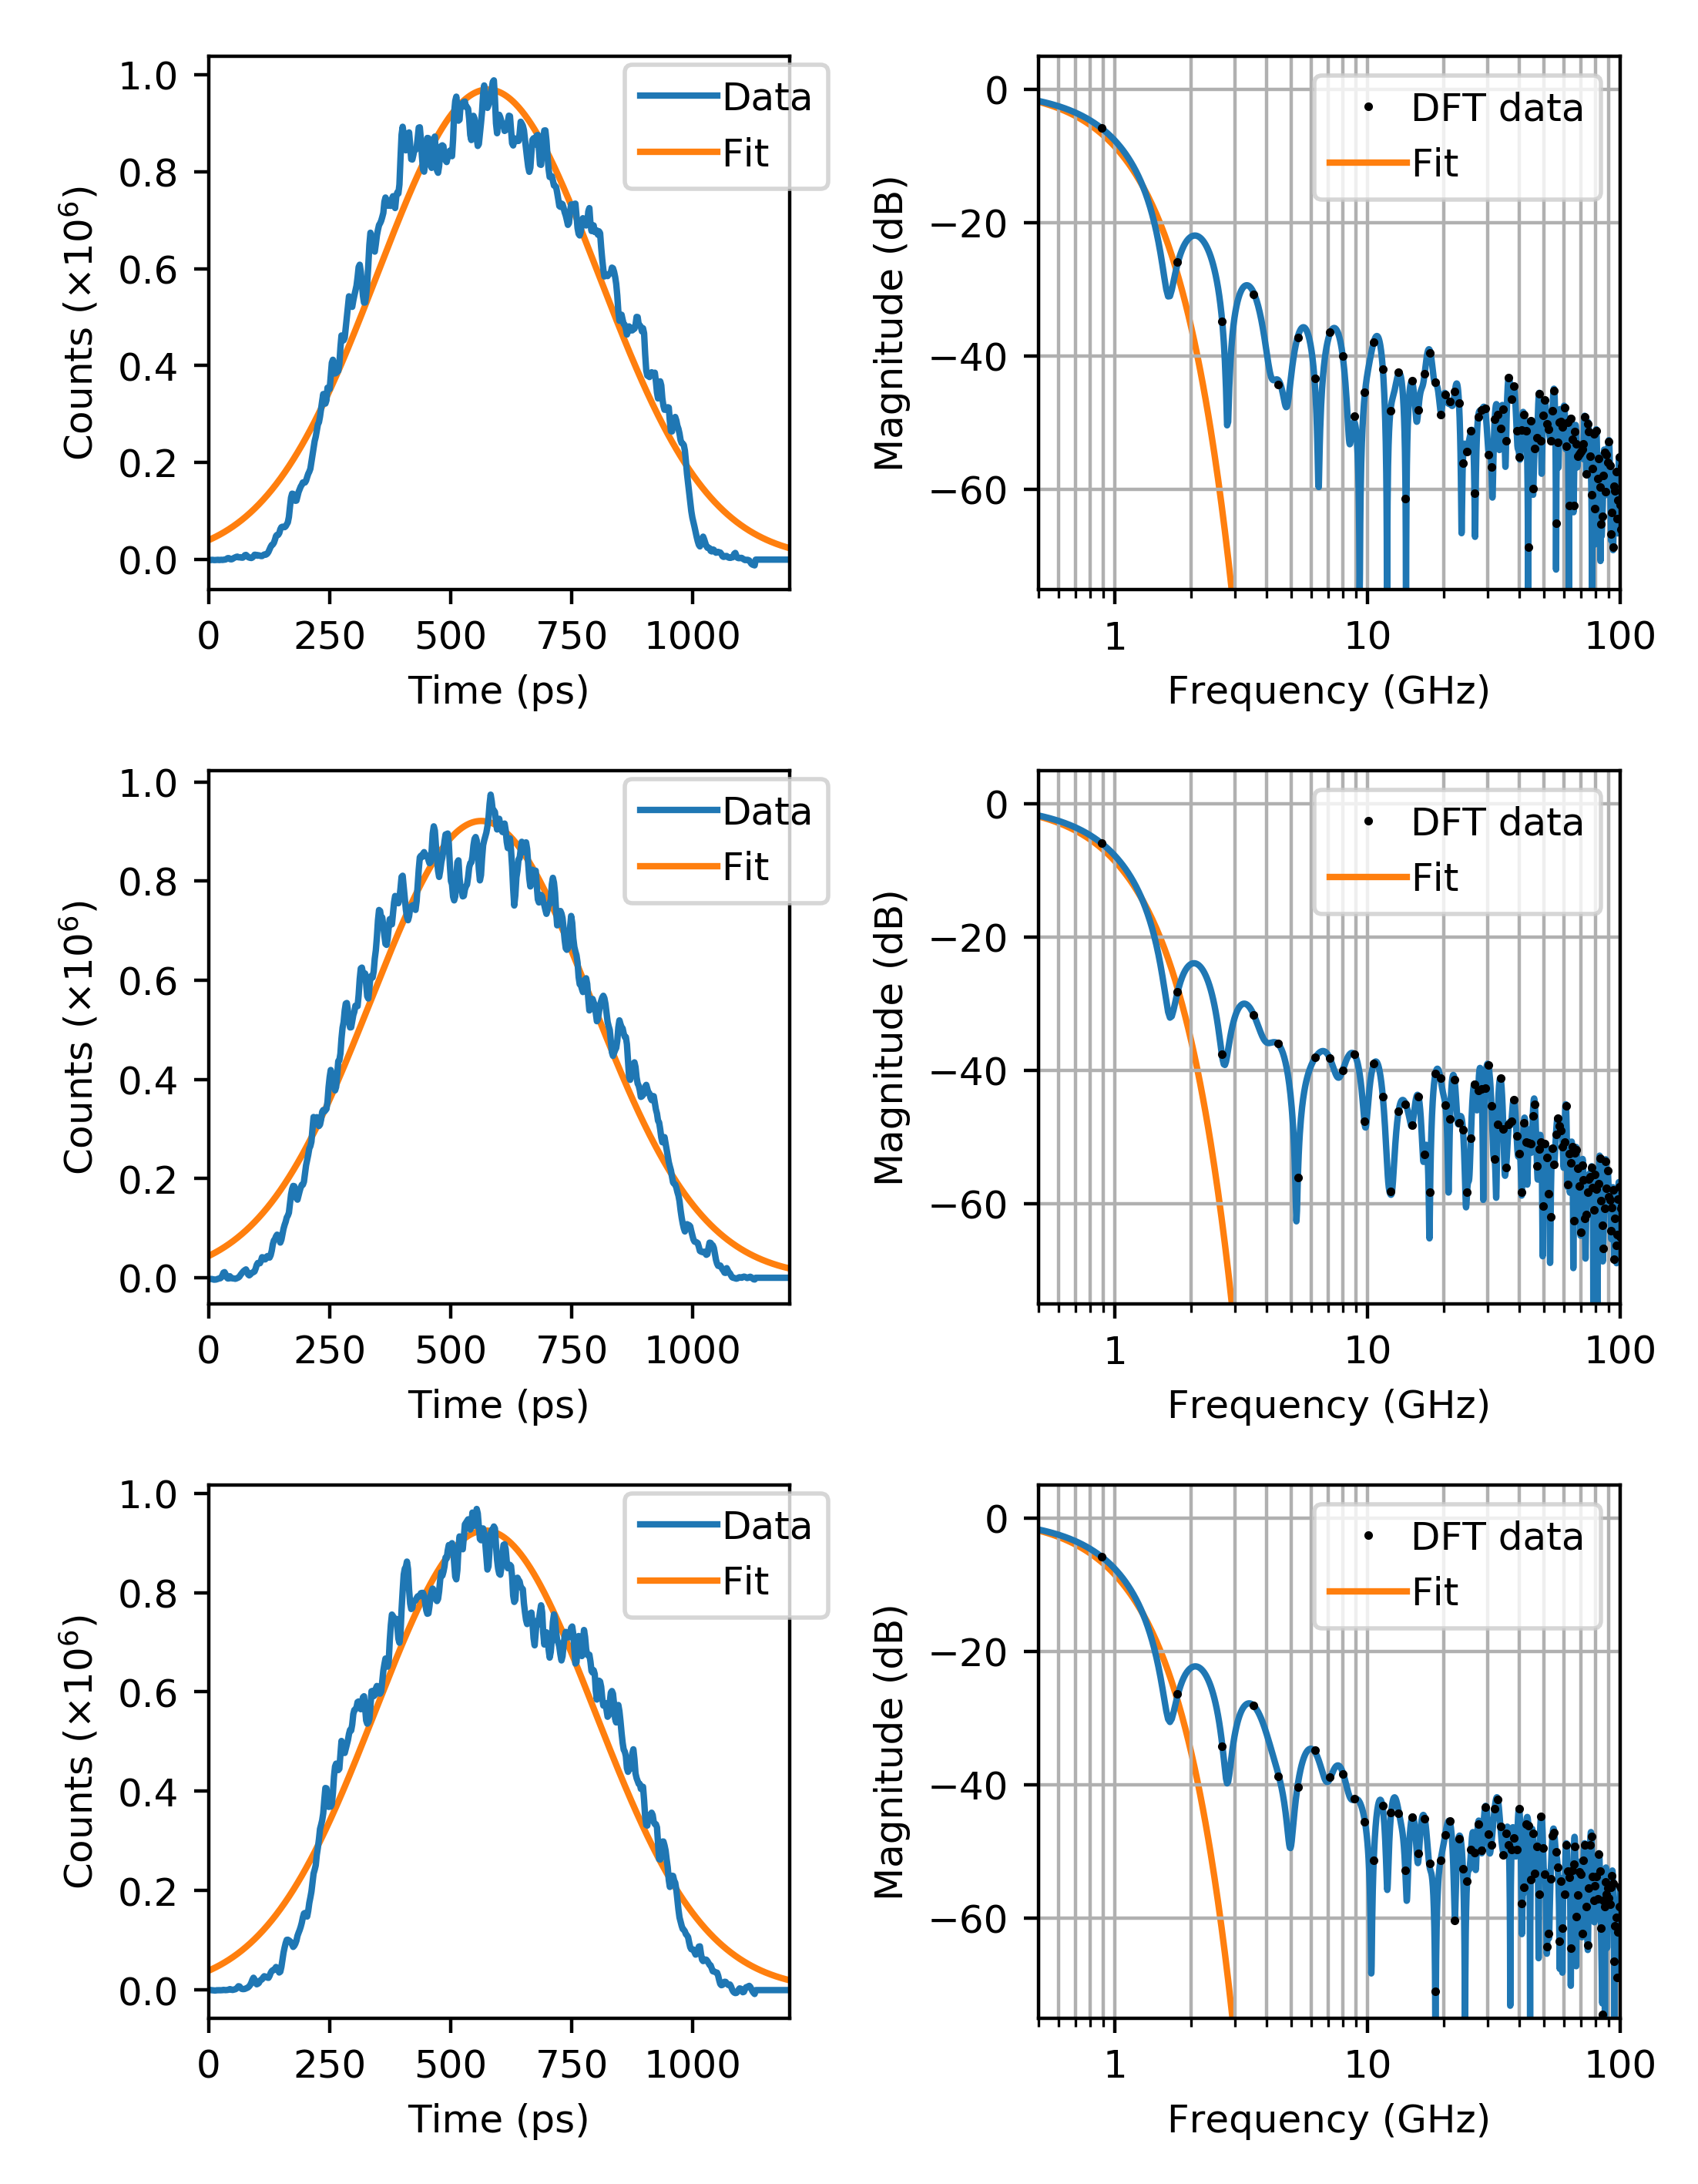
\includegraphics[scale=1, keepaspectratio]{pictures/profiles_fft}
\caption{Three examples of longitudinal proton bunch profiles measured with the streak camera together with Gaussian fits (orange lines). The plots to the left are in time domain while those to the right are their Fourier transforms. The spectrum is calculated for the raw camera image (black dots) and after increasing the frequency resolution (blue line).}
\label{fig:streak_profiles}
\end{figure}


\begin{figure}[!t]
\centering
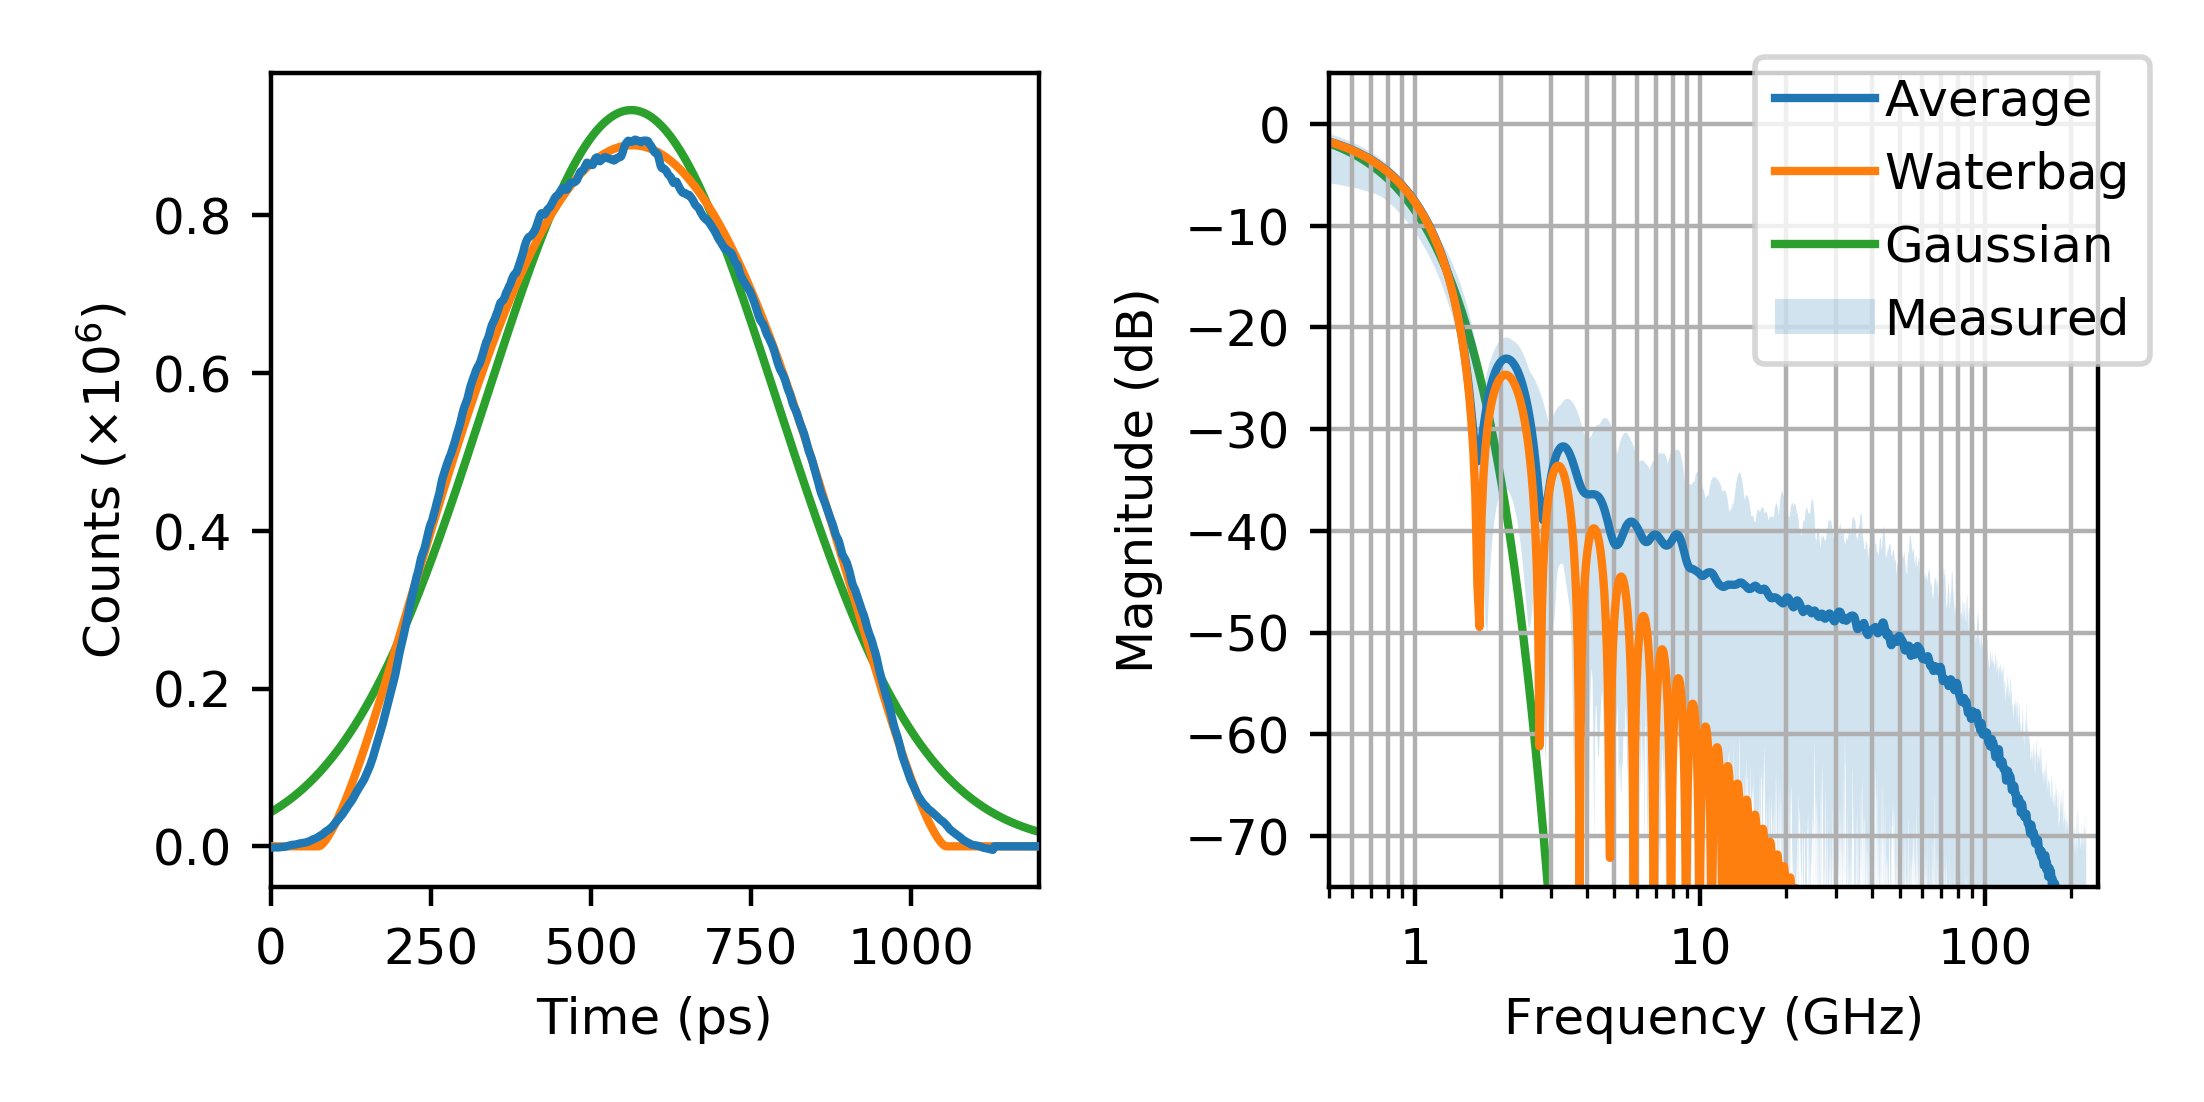
\includegraphics[scale=1, keepaspectratio]{pictures/AVG-vs-Waterbag}
\caption{Average beam profile (blue) in time domain (left) and its Fourier transform (right). The envelope of all recorded pulse spectra is shaded. Fits with the Gaussian and water-bag function are reported for comparison. The fit parameters are indicated in Table~\ref{tab:average_params}.}
\label{fig:fft_avg}

\vspace{3mm}

\begin{tabular}{l c c c c c c}
\toprule
        & Gaussian      &   Water bag\\
\midrule
Function    &  $A \, \text{exp} \left\{ \frac{1}{2}(\frac{x-\mu}{\sigma})^2   \right\}$       & $\frac{A}{t_b} \left( 1 - \left( \frac{2t}{t_b}   \right)^2  \right)^{3/2}$ \\\rule{0pt}{2.5ex}
$A$         &  $9553\pm10$      &   $8887\pm3$ \\
$\mu$ (ps)  &  $559.1\pm0.3$    &   $565.97\pm0.07$ \\
length (ps) &   $216.7\pm0.3$   &   $979.0\pm 0.2$ \\
\bottomrule
\end{tabular}
\captionof{table}{Fit parameters for the Gaussian and water bag functions. The bunch length is estimated as $\sigma$ for the Gaussian and $t_b$ for the water-bag function. It has to be noted that the two lengths are defined differently and, therefore, are not directly comparable. } \label{tab:average_params}


\end{figure}


The measurements indicate that the bunch spectrum contains significantly more power at high frequency than would be expected of a Gaussian bunch. It is therefore necessary to understand if this is a measurement artefact. The complicated nature of the streak camera measurement of OTR light makes it very difficult to precisely estimate the amount of introduced noise. However, some camera-induced noise can be reduced by averaging many profiles after aligning them in time. The profile center can be estimated as the point in the middle of the full width at half maximum (FWHM). A profile and its Fourier transform obtained by averaging 179 images are shown in Fig.~\ref{fig:fft_avg}. In the frequency domain plot, the envelope of all measured profiles is also shown around the average. Although a large part of the noise is removed, also most of the fine features are smoothed out. Two fits are also reported: Gaussian and using a `water-bag' function. The parameters for both fits are reported in Table~\ref{tab:average_params}. The former clearly reproduces the data poorly also for the average profile. The latter is defined as
\begin{equation}
f_\text{WB}(t, t_b, A)=
\begin{cases}
A \left( 1 - \left( \frac{2t}{t_b}   \right)^2  \right)^\frac{3}{2}   & |t| < \frac{t_b}{2}\\
0   &  |t| \ge \frac{t_b}{2}
\end{cases}\label{eq:waterbag}
\end{equation}
where $t_b$ is the bunch length measured at the base of the distribution and A is a normalisation parameter. In the frequency domain, the water bag fit shows a good agreement with the measurement up to $\sim$3~GHz. At higher frequencies, however, the measured proton spectrum decays much more slowly than for the fit. 


It is therefore not possible to precisely estimate the proton-bunch spectrum using streak-camera measurements at the frequencies of interest for this study, i.e. above $\sim 5$~GHz. However, the most pessimistic estimation of the proton spectrum is the envelope of the measurements, which includes the noise induced by the measurement. The water bag function fit is an approximation of the beam shape that works well up to $\sim$3~GHz. It can be assumed that the real beam spectrum lies between the measurement envelope and the water-bag fit. Furthermore, substantial shot-by-shot variations of the proton-bunch spectrum at high frequencies was measured. Therefore, the average proton spectrum will be taken into account in the BPM system design as this is the best data available at the moment. It has to be noted, however, that the proton bunch might contain a different amount of power at a given frequency than  accounted for using the average spectrum. 





\subsection[Implications for the system performance]{Implications for the system performance}

The AWAKE electron BPM system needs to work at a frequency  at which the electron beam signal is stronger than the proton one. As the working frequency choice is crucial for successful measurements, it is not sufficient to use the nominal parameters of 100-600~pC bunch charge and 1-4~ps bunch length \cite{Pepitone:2018gwl, Kim:2706086}.
An independent measurement of the AWAKE electron bunch length was carried out \cite{Mazzoni:courtesy}, and  is presented in Fig.~\ref{fig:bunch_length}. 

\begin{figure}[!t]
\centering
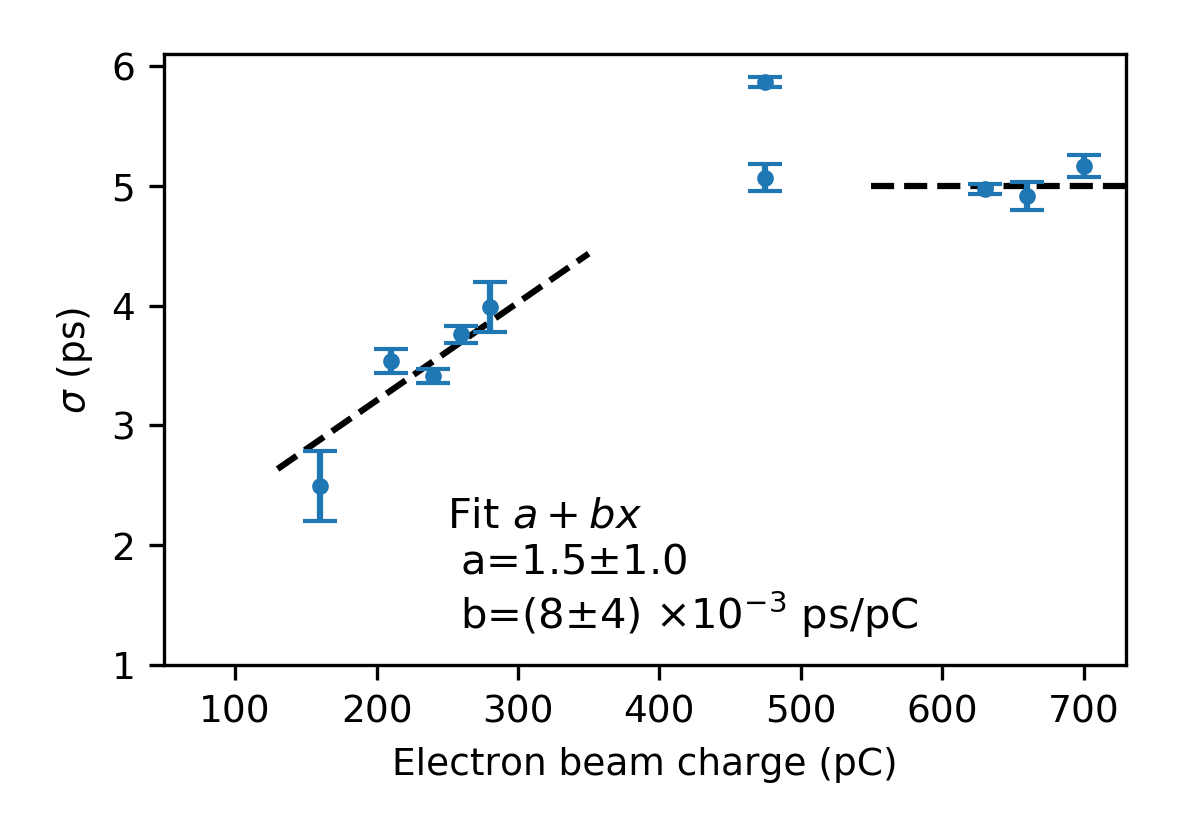
\includegraphics[scale=1.1, keepaspectratio]{pictures/measurement-echarge}
\caption{AWAKE electron bunch length (1 sigma) for different bunch-charge values. The measurement was carried out using the OTR screen light with the streak camera. The measurement error is its standard deviation obtained with three different processing methods. The dashed line on the left is a linear fit for charges smaller than 400~pC. The dashed line on the right indicates the mean value of the three measured points at charge larger than 500~pC \cite{Mazzoni:courtesy}.}
\label{fig:bunch_length}

\vspace{3mm}

\begin{tabular}{l c c c c c }
\toprule
Electron beam \\
\midrule
Charge (pC)& 100 & 200 & 300 & >500\\
$\sigma$ (ps)& 2.4 & 3.4 & 4 &	5\\
\bottomrule
\end{tabular}
\captionof{table}{Bunch-lengths obtained from measurements.} \label{tab:realistic_len}

\end{figure}
The measurement shows that the bunch length is correlated with the bunch charge up to $\sim400$~pC, and then it stabilises at 5~ps. A linear fit was performed on the data for charges smaller than 400~pC. The values in Table~\ref{tab:realistic_len} are obtained using the fit function, and serve as realistic design parameters of future beam instrumentation at AWAKE. It is not clear what caused the measurement discrepancy at 475~pC charge. However, other measurements indicate that 5~ps bunch length is achievable at this charge with appropriate injector settings. 

The measured electron beam parameters are compared with the average proton bunch spectrum in Fig.~\ref{fig:e_p_spectra} assuming that the longitudinal charge distribution in the electron bunch is Gaussian.
\begin{figure}[!h]
\centering
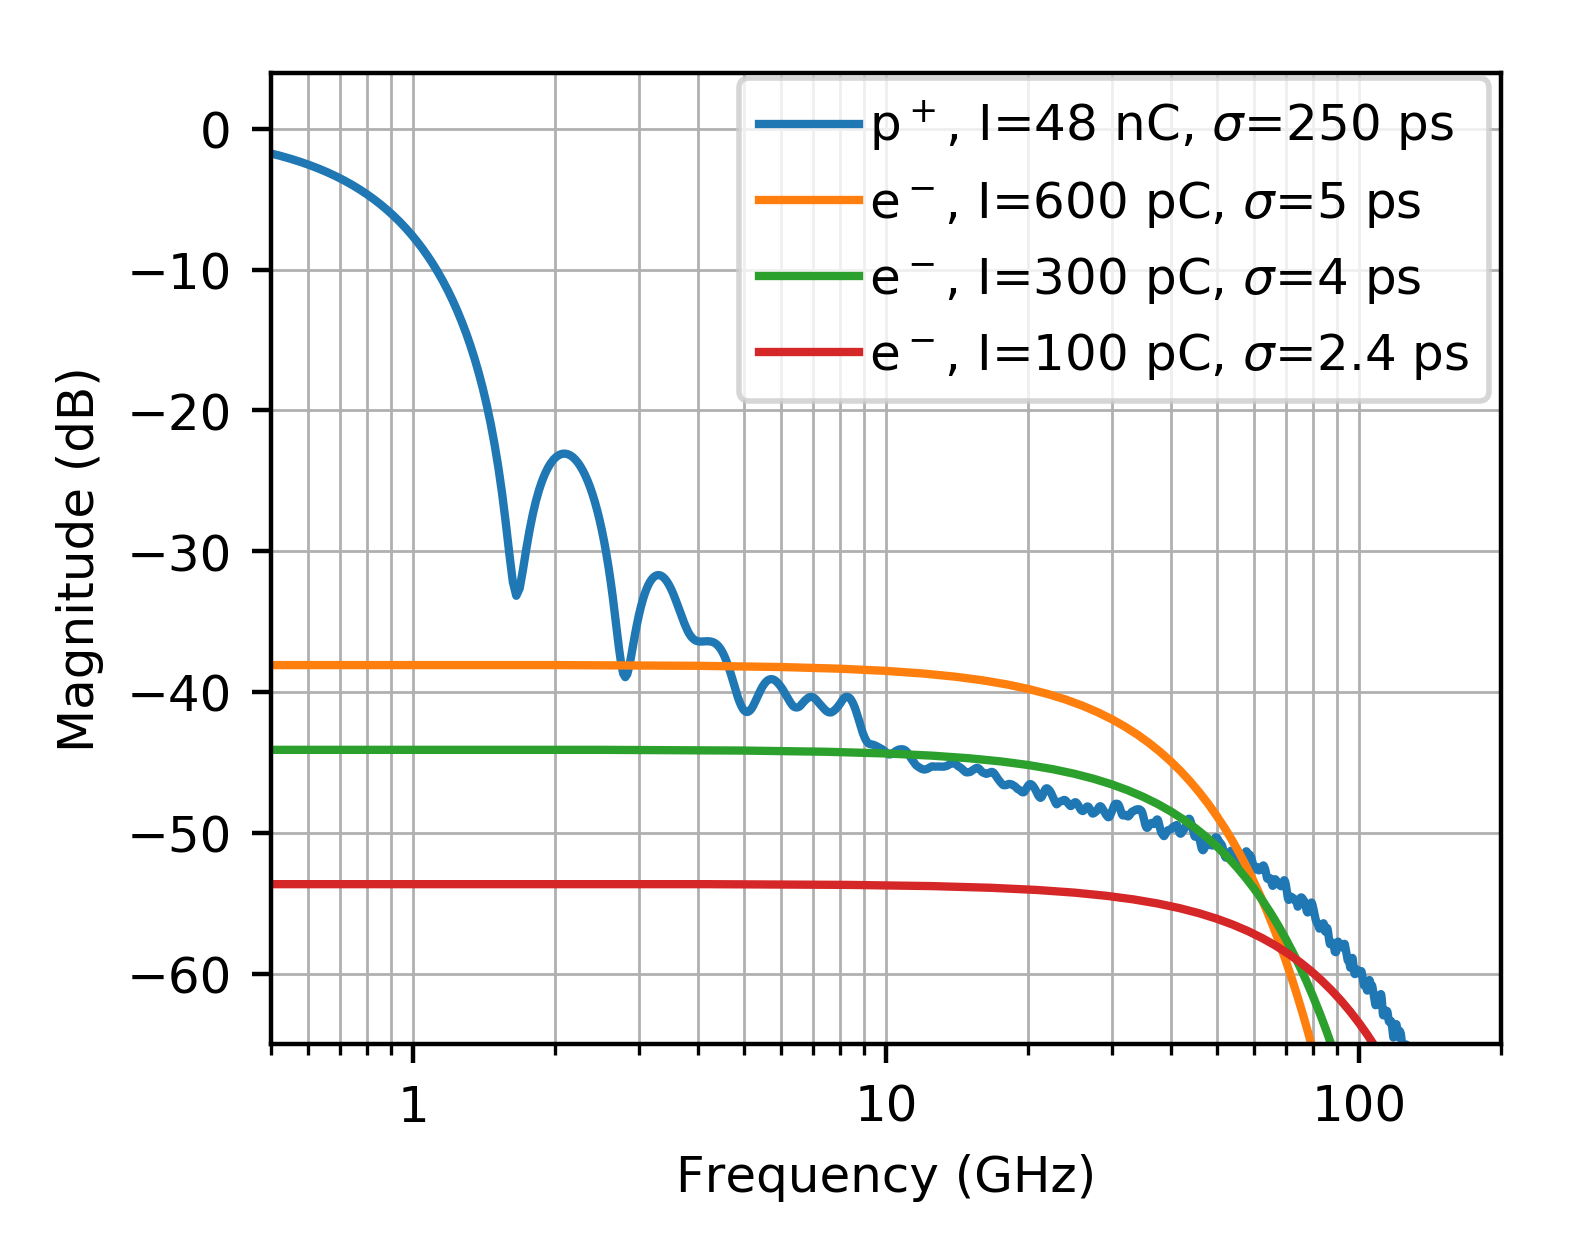
\includegraphics[scale=1, keepaspectratio]{pictures/e_p_spectra_real}
\caption{Comparison of spectra of the measured average proton bunch and electron bunch with different parameters. The electron bunch is assumed to follow a Gaussian longitudinal-charge distribution.}
\label{fig:e_p_spectra}
\end{figure}




The ratios of power carried by the electron and proton bunches at different frequencies are shown in Fig.~\ref{fig:e_p_ratio}. For the lowest electron bunch charge of 100~pC, the electron bunch signal is stronger than the proton one only at a frequency above 100~GHz. For charges of 300~pC and above, the electron signal becomes stronger than the proton in the range between 15 and 40~GHz. Also, this analysis shows that there is no substantial difference between carrying out the measurement at 20 or 30~GHz. For technical and cost reasons a lower frequency is preferable, hence an operating frequency of the electron BPM system of around 20~GHz appears to be the optimal choice. 

\newpage

\begin{figure}[!t]
\centering
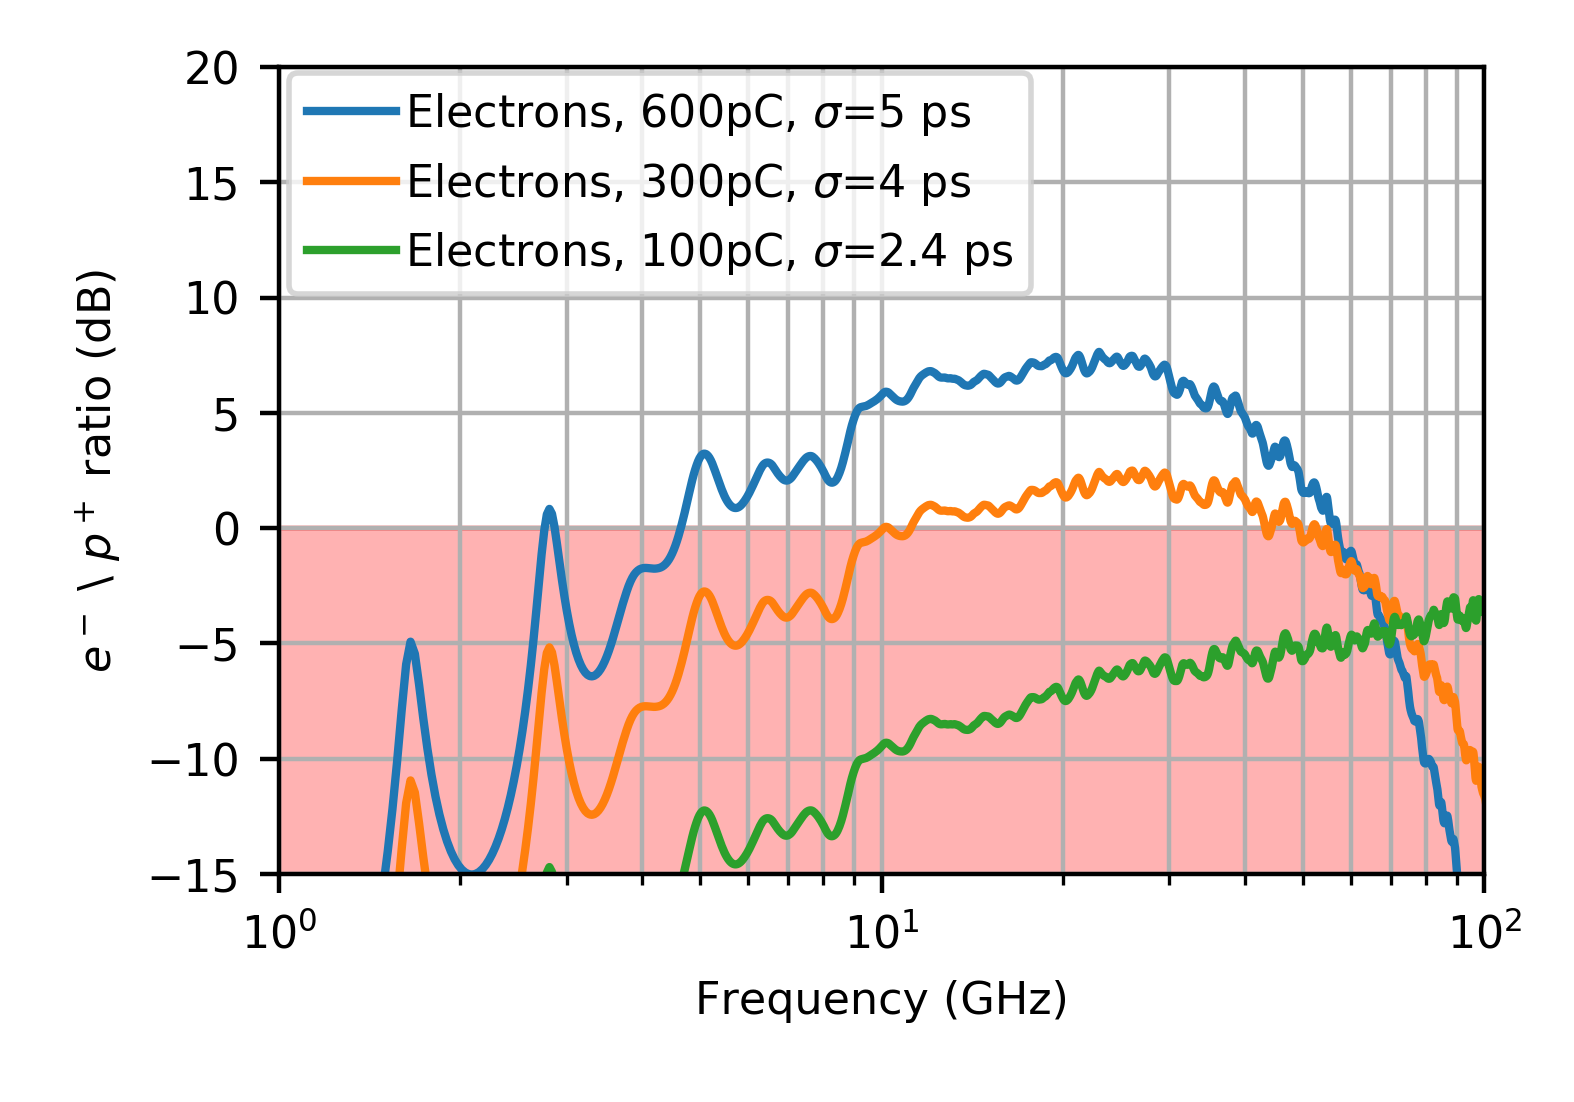
\includegraphics[scale=1.1, keepaspectratio]{pictures/e_p_ratio_real}
\caption{Ratios between the measured average proton-bunch and the electron-bunch spectra for different electron-beam parameters. The red area marks the region where the proton signal is more intense than the electron one.}
\label{fig:e_p_ratio}
\end{figure}




In summary, the position measurement of a shorter and less intense electron beam can be achieved in the  presence of a more intense and longer proton beam, provided that the measurement is carried out in a frequency band where the signal from the electron beam is dominant. An analytical model for Gaussian beams has been presented. The impact of the non-Gaussian shape of the AWAKE proton drive beam was discussed, although the available data do not allow a precise estimate of the proton beam spectrum in the tens-of-GHz regime due to the nature of the streak-camera measurement. However, an estimation using the average proton-beam longitudinal profile was derived, showing that the AWAKE nominal electron-beam signal is dominant over the proton-beam signal in the 20-30~GHz range. Detecting the beam position in this high-frequency range presents major technical difficulties. An innovative approach to solve this problem based on the emission of Cherenkov Diffraction Radiation is presented in Chapter~\ref{chapter:CLEAR_test}. 